\documentclass[12pt,openany,twoside,a4paper]{abntex2}
\usepackage{indentfirst}

\usepackage{tikz}
\usetikzlibrary{positioning}
\usetikzlibrary{shapes}
\usetikzlibrary{calc}
\usetikzlibrary{tikzmark}
\usetikzlibrary{fit}

\usepackage{multicol}
\usepackage{mathtools}
\usepackage{amsmath}
\usepackage{amsfonts}
\usepackage{framed}
\usepackage{graphicx}
\usepackage{titlesec}
\usepackage{xcolor}
\usepackage{import}
\usepackage{ulem}
\usepackage[boxed, portuguese, portuguesekw]{algorithm2e}
\SetKwProg{Fn}{Função}{}{fim}

\usepackage{listings}
\definecolor{mygreen}{rgb}{0,0.6,0}
\definecolor{mygray}{rgb}{0.5,0.5,0.5}
\definecolor{mymauve}{rgb}{0.58,0,0.82}

\lstset{ 
  backgroundcolor=\color{white},   % choose the background color; you must add \usepackage{color} or \usepackage{xcolor}; should come as last argument
  basicstyle=\ttfamily,        % the size of the fonts that are used for the code
  breakatwhitespace=false,         % sets if automatic breaks should only happen at whitespace
  breaklines=true,                 % sets automatic line breaking
  captionpos=b,                    % sets the caption-position to bottom
  commentstyle=\color{mygreen},    % comment style
  deletekeywords={...},            % if you want to delete keywords from the given language
  escapeinside={\%*}{*)},          % if you want to add LaTeX within your code
  extendedchars=true,              % lets you use non-ASCII characters; for 8-bits encodings only, does not work with UTF-8
  firstnumber=1,                   % start line enumeration with line 1
  frame=single,	                   % adds a frame around the code
  keepspaces=true,                 % keeps spaces in text, useful for keeping indentation of code (possibly needs columns=flexible)
  keywordstyle=\color{blue},       % keyword style
  language=Python,                 % the language of the code
  morekeywords={*,...},            % if you want to add more keywords to the set
  numbers=none,                    % where to put the line-numbers; possible values are (none, left, right)
  numbersep=5pt,                   % how far the line-numbers are from the code
  numberstyle=\tiny\color{mygray}, % the style that is used for the line-numbers
  rulecolor=\color{black},         % if not set, the frame-color may be changed on line-breaks within not-black text (e.g. comments (green here))
  showspaces=false,                % show spaces everywhere adding particular underscores; it overrides 'showstringspaces'
  showstringspaces=false,          % underline spaces within strings only
  showtabs=false,                  % show tabs within strings adding particular underscores
  stepnumber=1,                    % the step between two line-numbers. If it's 1, each line will be numbered
  stringstyle=\color{mymauve},     % string literal style
  tabsize=2,	                   % sets default tabsize to 2 spaces
  title=\lstname                   % show the filename of files included with \lstinputlisting; also try caption instead of title
}

\author{Marcio Lima Inácio}
\title{Introdução à Otimização Combinatória Aplicada}

\begin{document}
\makeatletter
\def\maketitle{%
  \null
  \thispagestyle{empty}%
  \vfill
  \begin{flushright}\leavevmode
    \normalfont
    {\@author\par}%
    \hrulefill\par
    {\huge\@title\par}%
    \vskip 1cm
  \end{flushright}%
  \vfill
  \null
}

\renewcommand{\thesection}{\@arabic\c@section}
\makeatother

\makechapterstyle{aula}{
  \chapterstyle{default}
  \renewcommand*{\chaptitlefont}{\normalfont\Large\scshape}
  \renewcommand*{\chapterheadstart}{}
  \renewcommand*{\printchaptername}{\chaptitlefont Semana}
  \renewcommand*{\afterchapternum}{\vskip\onelineskip \hrule\vskip\onelineskip}
  \renewcommand*{\printchapternum}{\chaptitlefont \thechapter}
  \renewcommand{\printchaptertitle}[1]{\raggedleft\chaptitlefont ##1}
  % \renewcommand*{\afterchaptertitle}{\vskip\onelineskip \hrule\vskip\onelineskip}
}
\chapterstyle{aula}

\titleformat{\section}[block]
{\filcenter\large\sffamily\bfseries}
{Aula \thesection}
{1em}{}

\newenvironment{example}
{
  \begin{framed}
    }
    {
  \end{framed}
}

\maketitle

\mainmatter

\chapter{Introdução}

\section{Otimização Combinatória}

Definição: Problema de Otimização

\begin{itemize}
    \item Entrada (instância)
    \item Conjunto de soluções viáveis
          \begin{itemize}
              \item Soluções válidas
              \item Respeitam as restrições do problema
          \end{itemize}
\end{itemize}

Quero achar a melhor solução

\begin{itemize}
    \item Função objetivo
          \begin{itemize}
              \item Asssocia um valor real a cada solução viável
          \end{itemize}
\end{itemize}

Melhor: maximização ou minimização -- De acordo com a função objetivo

Otimização Combinatória

\begin{itemize}
    \item Variáveis discretas
    \item O conjunto de soluções viáveis é finito
\end{itemize}

\begin{example}
    Problema do escalonamento

    Dadas $n$ tarefas, cada uma com uma duração, alocá-las em $m$ máquinas minimizando a maior soma de tempos (\textit{makespan}).

    \vspace{\baselineskip}
    Instâncias

    \qquad $m = 2$
    \begin{center}
        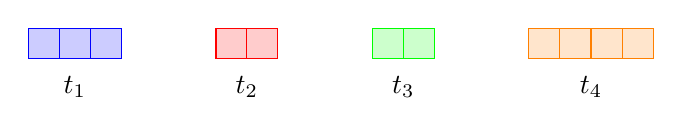
\begin{tikzpicture}[tempo/.style 2 args={rectangle split,
                        rectangle split horizontal, draw=#2, rectangle split parts=#1, fill=#2!20, outer sep=1mm}]
            \node[tempo={3}{blue}, label=below:$t_1$] (t1) at (0, 0) {};
            \node[tempo={2}{red}, label=below:$t_2$] (t2) [right=of t1] {};
            \node[tempo={2}{green}, label=below:$t_3$] (t3) [right=of t2] {};
            \node[tempo={4}{orange}, label=below:$t_4$] (t4) [right=of t3] {};
        \end{tikzpicture}
    \end{center}

    Exemplos de soluções

    \begin{multicols}{2}
        \begin{tabular}{l|l}
            $M_1$ & \tikzmark{1m11} \\
            $M_2$ & \tikzmark{1m21} \\
        \end{tabular}

        \begin{tikzpicture}[remember picture, tempo/.style 2 args={rectangle split, rectangle split horizontal, overlay, draw=#2, rectangle split parts=#1, fill=#2!20, anchor=west}, node distance=1pt]
            \node[tempo={3}{blue}] (t1) at (pic cs:1m11) {};
            \node[tempo={4}{orange}] (t4) [right=of t1] {};
            \node[tempo={2}{red}] (t2) at (pic cs:1m21) {};
            \node[tempo={2}{green}] (t3) [right=of t2] {};
        \end{tikzpicture}

        \begin{center}
            \textit{makespan} = $7$
        \end{center}

        \columnbreak

        \begin{tabular}{l|l}
            $M_1$ & \tikzmark{1m12} \\
            $M_2$ & \tikzmark{1m22} \\
        \end{tabular}

        \begin{tikzpicture}[remember picture, tempo/.style 2 args={rectangle split, rectangle split horizontal, overlay, draw=#2, rectangle split parts=#1, fill=#2!20, anchor=west}, node distance=1pt]
            \node[tempo={3}{blue}] (t1) at (pic cs:1m12) {};
            \node[tempo={2}{red}] (t2) [right=of t1] {};
            \node[tempo={4}{orange}] (t4) at (pic cs:1m22) {};
            \node[tempo={2}{green}] (t3) [right=of t4] {};
        \end{tikzpicture}

        \begin{center}
            \textit{makespan} = 6
        \end{center}
    \end{multicols}
\end{example}

\section{Definições básicas}

\subsection{Grafos}

Estrutura matemática que representa relacionamentos par-a-par (arestas) entre objetos (vértices).

Formalização: $G = (V, E)$

\qquad $V =$ conjunto de vértices

\qquad $E =$ conjunto de arestas

$E$ é um conjunto de pares.

\begin{example}
    \begin{multicols}{2}
        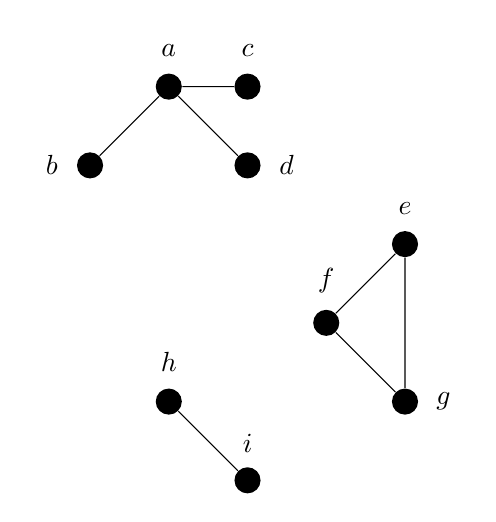
\begin{tikzpicture}[every node/.style={circle, fill}]
            \node[label=$a$] (a) at (0, 0) {};
            \node[label=left:$b$] (b) at (-1, -1) {};
            \node[label=$c$] (c) at (1, 0) {};
            \node[label=right:$d$] (d) at (1, -1) {};
            \draw (a) -- (b) (a) -- (c) (a) -- (d);

            \node[label=$e$] (e) at (3, -2) {};
            \node[label=$f$] (f) at (2, -3) {};
            \node[label=right:$g$] (g) at (3, -4) {};
            \draw (e) -- (f) -- (g) -- (e);

            \node[label=$h$] (h) at (0, -4) {};
            \node[label=$i$] (i) at (1, -5) {};
            \draw (h) -- (i);
        \end{tikzpicture}

        \columnbreak

        $V = \{a, b, c, d, e, f, g, h, i\}$

        $E = \{(a, b), (a, c), (a, d), (h, i), \dots\}$
    \end{multicols}
\end{example}

Tipos comuns de grafos

\begin{itemize}
    \item Caminho
          \begin{itemize}
              \item Conexo
              \item Não possui bifurcação
          \end{itemize}
          \begin{example}
              \begin{center}
                  \tikz[every node/.style={circle, fill}]
                  \draw (0, 0) node {} -- (1, 0) node {} -- (2, 0) node {} -- (3, 1) node {} -- (4, 0) node {} -- (4, -1) node {} -- (5, 0) node {};
              \end{center}
          \end{example}
    \item Circuito
          \begin{itemize}
              \item Fecha o ciclo
          \end{itemize}
          \begin{example}
              \begin{center}
                  \tikz[every node/.style={circle, fill}]
                  \draw (0, 0) node(a) {} -- (1, 1) node {} -- (2, 1) node {} -- (3, 0) node {} -- (3, -1) node {} -- (2, -2) node {} -- (1, -1) node {} -- (a);
              \end{center}
          \end{example}
    \item Completo
          \begin{itemize}
              \item Todos os nós conectados entre si
              \item Representado por $K_n$, sendo $n$ o número de vértices
          \end{itemize}
          \begin{example}
              \begin{center}
                  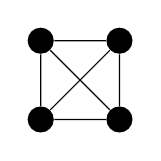
\begin{tikzpicture}[every node/.style={circle, fill}]
                      \node (a) at (0, 0) {};
                      \node (b) at (1, 0) {};
                      \node (c) at (0, 1) {};
                      \node (d) at (1, 1) {};

                      \draw (a) -- (b) (a) -- (c) (a) -- (d);
                      \draw (b) -- (c) (b) -- (d) -- (c);
                  \end{tikzpicture}
              \end{center}
          \end{example}
    \item Bipartidos
          \begin{itemize}
              \item Dois subconjuntos de vértices sem arestas entre split
              \item Tipos de entidades distintas
          \end{itemize}
          \begin{example}
              \begin{center}
                  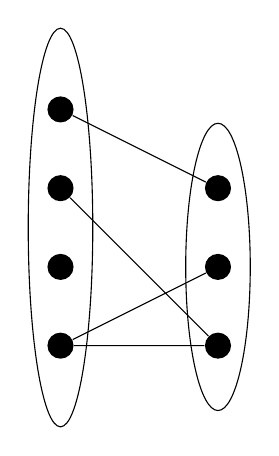
\begin{tikzpicture}[n/.style={circle, fill}]
                      \node[n] (a) at (0, 0) {};
                      \node[n] (b) at (0, 1) {};
                      \node[n] (c) at (0, 2) {};
                      \node[n] (d) at (0, 3) {};

                      \node[n] (e) at (2, 0) {};
                      \node[n] (f) at (2, 1) {};
                      \node[n] (g) at (2, 2) {};

                      \node[draw, ellipse, fit=(a)(b)(c)(d)] {};
                      \node[draw, ellipse, fit=(e)(f)(g)] {};

                      \draw (a) -- (e) -- (c) (a) -- (f) (d) -- (g);
                  \end{tikzpicture}
              \end{center}
          \end{example}
    \item Árvores
          \begin{itemize}
              \item Grafos conexos e acíclicos
              \item Caminhos são um tipo específico de árvore
              \item Para qualquer par de nós $a$ e $b$, existe um único caminho conectando $a$ a $b$
          \end{itemize}
          \begin{example}
              \begin{center}
                  \tikz[every node/.style={circle, fill}]
                  \draw (0, 0) node {} -- (1, 0) node (a) {} -- (2, 1) node {} (a) -- (2, -1) node {} -- (3, 0) node (b) {} -- (4, 1) node {} (b) -- (4, 0) node {} (b) -- (4, -1) node {};
              \end{center}
          \end{example}
\end{itemize}

Os grafos podem ser \underline{orientados} (ou dirigidos) ou \underline{não-orientados}. No caso dos grafos orientados, as arestas (também chamadas de arcos) têm uma direção.

Os grafos também podem ter pesos (ou custos) associados às arestas.

\begin{example}
    \begin{center}
        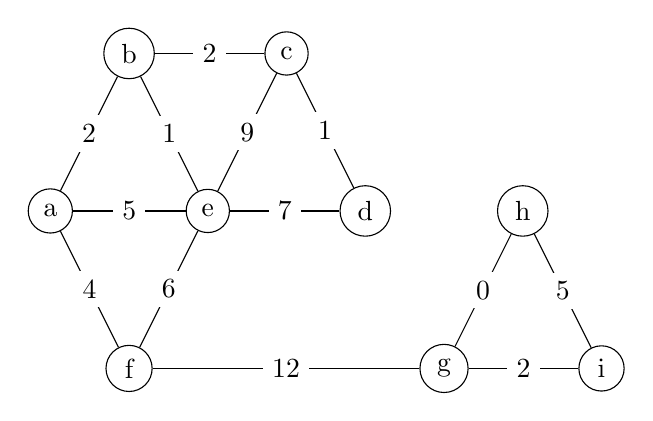
\begin{tikzpicture}[every node/.style={fill=white}, n/.style={circle, draw}]
            \node[n] (a) at (0, 0) {a};
            \node[n] (b) at (1, 2) {b};
            \node[n] (c) at (3, 2) {c};
            \node[n] (d) at (4, 0) {d};
            \node[n] (e) at (2, 0) {e};
            \node[n] (f) at (1, -2) {f};
            \node[n] (g) at (5, -2) {g};
            \node[n] (h) at (6, 0) {h};
            \node[n] (i) at (7, -2) {i};

            \draw (a) edge node {2} (b) edge node {5} (e) edge node {4} (f)
            (b) edge node {2} (c) edge node {1} (e)
            (c) edge node {1} (d) edge node {9} (e)
            (d) edge node {7} (e)
            (e) edge node {6} (f)
            (f) edge node {12} (g)
            (g) edge node {0} (h) edge node {2} (i)
            (h) edge node {5} (i);
        \end{tikzpicture}
    \end{center}
\end{example}

Os pesos são formalizados como uma função separada: $f: E \mapsto \mathbb{R}$.

\subsection{Análise de algoritmos}

Mostra que

\begin{itemize}
    \item Um algoritmo está correto
    \item Estimar o tempo de execução
\end{itemize}

É uma análise matemática, então \underline{não é preciso implementar o algoritmo}.

Notação assintótica: termos de menor ordem e constantes são de desconsiderados.

$20n^2 + 500n \rightarrow O(n^2)$

\section{Exemplos de problemas}

\subsection{Árvore de Steiner}

\begin{itemize}
    \item \textbf{Entrada:} $G = (V, E)$ com $V = R \cup S$, sendo $R$ terminais e $S$ vértices de Steiner, e função $w$ de peso na arestas.
    \item \textbf{Soluções viáveis:} árvores que conectam todos os vértices em $R$.
    \item \textbf{Função objetivo:} soma dos pesos das arestas na árvore.
    \item \textbf{Objetivo:} enconctrar uma árvore de peso mínimo.
\end{itemize}

\subsection{\textit{Bin Packing}/Empacotamento}

\begin{itemize}
    \item \textbf{Entrada:} conjunto $L = \{1,\dots,n\}$ de itens retangulares, item $i$ com largura $w_i$ e altura $h_i$, largura $W$ e altura $H$ do recipiente retangular.
    \item \textbf{Soluções viáveis:} partição $L_1, L_2, \dots, L_q$ de $L$ tal que os itens em $L_k$ cabem num recipiente $W \times H$.
    \item \textbf{Função objetivo:} número $q$ de recipientes (\textit{bins}) utilizados.
    \item \textbf{Objetivo:} encontrar solução de custo mínimo.
\end{itemize}

\subsection{Caixeiro Viajante (TSP - \textit{Traveling Salesman Problem})}

\begin{itemize}
    \item \textbf{Entrada:} $G = (V, E)$ e função $w$ de peso nas arestas.
    \item \textbf{Soluções viáveis:} circuitos hamiltonianos (passam por todos os vértices sem repetição) de $G$.
    \item \textbf{Função objetivo:} soma dos pesos das arestas do circuito.
    \item \textbf{Objetivo:} encontrar o circuito de menor custo
\end{itemize}

\subsection{Problema da Mochila}

\begin{itemize}
    \item \textbf{Entrada:} conjunto de $n$ itens, cada item $i$ tem peso $w_i$ e valor $v_i$ e tamanho $W$ da mochila.
    \item \textbf{Soluções viáveis:} conjuntos de itens $S \subseteq \{1,\dots,n\}$ com $\sum_{i \in S} w_i \leq W$.
    \item \textbf{Função objetivo:} soma dos valores dos itens em $S$.
    \item \textbf{Obejtivo:} encontrar uma solução de valor máximo.
\end{itemize}

\section{Dificuldades}

Primeira abordarem de resolução de problemas: busca por força bruta.

O espaço de busca é finito, então dá para enumerar todas as soluções guardando a melhor encontrada. \underline{Com tempo suficiente}, resolve o problema.

Mas não explora as estruturas combinatórias do problema. $\to$ Muito esforço.

Com um espaço muito grande, fica inviável usar.

\begin{example}
    No TSP qualquer sequência dos $n$ vértices é candidata a solução.

    \vspace{\baselineskip}
    Algoritmo:
    \begin{enumerate}
        \item Gere as $n!$ sequências de vértices
        \item Cada sequência é um circuito hamiltoniano
        \item Calcule seu custo e compare com o melhor já encontrado
    \end{enumerate}

    \textbf{São $\mathbf{(n-1)!}$ sequências no espaço de busca.}
\end{example}

\begin{example}
    No problema da mochila, qualquer subconjunto dos $n$ elementos é candidato a solução.

    \vspace{\baselineskip}
    Algoritmo:
    \begin{enumerate}
        \item Gere os $2^{n}$ possíveis subconjuntos
        \item Para cada um, teste se os itens cabem na mochila $\to$ \underline{Viabilidade}
        \item Se couberem, calcule o custo da soluçào e compare com o melhor já encontrado
    \end{enumerate}

    \textbf{Crescimento exponencial}
\end{example}

\subsection{Complexidade}

\begin{itemize}
    \item Algoritmo eficiente: complexidade de tempo no pior caso é polinomial no tamanho $n$ da entrada $\to O(n^{k})$ com $k$ constante.
    \item Problemas de decisão: Problemas com resposta \underline{sim} ou \underline{não}.
\end{itemize}

Classes de problemas:

\begin{itemize}
    \item \textbf{Classe P:} problemas de decisão que possuem algoritmos eficientes.
    \item \textbf{Classe NP:} problemas de decisão cuja solução ("resposta \underline{sim}") pode ser \underline{verificada} em tempo polinomial.
    \item \textbf{Classe NP-Completo}: problemas Q tais que $\mathrm{Q} \in \mathrm{NP}$ e todo problema \underline{em NP} é redutível a Q.
\end{itemize}

\textbf{Redução}

Um problema A é redutível a B se podemos utilizar um algoritmo que resolve B para resolver A, ou seja, \underline{B é pelo menos tão difícil quanto A}.

Não há um certificado de dificuldade absoluto: "esse problema não é possíel de resolver". Existe a dificuldade relativa: "esse problema é tão complexo quanto aquele".

\begin{itemize}
    \item \textbf{Classe NP-Difícil}: problemas Q tais que todo problema em NP é redutível a Q. Esses problemas não precisam ser necessariamente NP ($\neq$ NP-Completo).
\end{itemize}

\subsection{Abordagens}

Se $\mathrm{P} \neq \mathrm{NP}$, não é possível ter algoritmos para problemas NP-Difíceis que:
\begin{itemize}
    \item Encontrem soluções ótimas
    \item Em tempo polinomial
    \item Para qualquer entrada
\end{itemize}

Tem que abrir mão de alguma característica

\begin{itemize}
    \item Métodos exatos
          \begin{itemize}
              \item Não funcionam em tempo hábil (exponencial ou superpolinomial)
              \item Ao contrário da força bruta, explora as estruturas combinatórias para eliminar pedaços do espaço de busca para facilitar
          \end{itemize}
    \item Heurísticas
          \begin{itemize}
              \item Não encontra necessariamente soluções ótimas
              \item Procura soluções ``boas o bastante''
              \item Avaliação empírica com o uso de \textit{benchmarks} de instâncias
          \end{itemize}
    \item Algoritmos de aproximação
          \begin{itemize}
              \item Não encontra necessariamente soluções ótimas (subconjunto das heurísticas)
              \item Garantia de que o algoritmo é polinomial
              \item Garantia de que o resultado vai estar dentro de uma margem de erro da solução ótima
          \end{itemize}
    \item Parametrização
          \begin{itemize}
              \item Não funciona para todas as instâncias
              \item Um parâmetro é fixado
              \item Garantia de encontrar a solução ótima para as instâncias com o parâmetro fixo
          \end{itemize}
\end{itemize}

\section{Métodos exatos}

\begin{itemize}
    \item Procuram a solução ótima
    \item Considera as estruturas combinatórias do problema $\to$ Diferença da força bruta
    \item Não garante tempo polinomial no pior caso (Problemas NP-Difíceis)
\end{itemize}

Exemplos de métodos exatos

\begin{itemize}
    \item Algoritmos gulosos
    \item Programação dinâmica
    \item \textbf{\textit{Branch and bound}}
    \item \textbf{Programação linear / Programação linear inteira}
    \item Programação por restrições $\times$
\end{itemize}

\subsection{Algoritmos gulosos}

Realizam decisões melhores em curto prazo, esperando que isso leve ao resultado ótimo.

Existem casos que um algoritmo guloso resolve o problema em tempo polinomial para todas as instâncias. Exemplos:

\begin{itemize}
    \item Caminho mínimo $\to$ Dijkstra
    \item MST $\to$ Prim e Kruskal
    \item Compressão de Dados $\to$ Huffman
    \item Mochila Fracionária
\end{itemize}

Para problemas NP-Difíceis, dá para usar algoritmos gulosos \underline{como heurísticas}.

\subsubsection{Mochila Fracionária}

Os itens que são colocados na mochila podem ser divisíveis. Pode pegar frações de itens.

Objetivo: pegar os itens com o maior custo-benefício. Razão $\frac{\mathrm{valor}}{\mathrm{peso}}$. Garantir que ninguém melhor está fora da mochila.

\begin{example}
    \begin{multicols}{2}

        $W = 50$

        $v_1 = 60$ \hspace{10pt} $w_1 = 10$ \hspace{10pt} $\frac{v_1}{w_1} = 6$

        $v_2 = 100$ \hspace{10pt} $w_2 = 20$ \hspace{10pt} $\frac{v_2}{w_2} = 5$

        $v_3 = 120$ \hspace{10pt} $w_3 = 30$ \hspace{10pt} $\frac{v_3}{w_3} = 4$

        \columnbreak

        Ordem decrescente: 1, 2, 3

        Fração item 1: $100\%$

        Espaço livre: $50 - 10 = 40$

        Fração item 2: $100\%$

        Espaço livre: $40 - 20 = 20$

        Fração item 3: $\frac{20}{30} = 66\%$

        Espaço livre: $20 - 20 = 0$
    \end{multicols}
\end{example}

\begin{algorithm}
    \SetAlgoLined
    \SetKwFunction{MochilaFrac}{MochilaFrac}

    \Fn{\MochilaFrac{$n: \mathrm{itens}$, $w: \mathrm{peso}$, $v: \mathrm{valor}$, $W: \mathrm{capacidade}$}}{

        Ordene e renomeie os itens para que $\frac{v_1}{w_1} \geq \frac{v_2}{w_2} \geq \cdots \geq \frac{v_n}{w_n}$\;

        Seja $q$ um inteiro tal que $X = \sum_{i=1}^{q}w_i \leq W$ e $\sum_{i=1}^{q+1} w_i > W$

        Cabe ainda uma fração $\frac{W-X}{w_{q+1}}$ do item $q + 1$

        \Retorna{$v_1 + v_2 + \dots + v_q + v_{q+1} \frac{W-X}{w_{q+1}}$}
    }
\end{algorithm}

\subsection{\textit{Branch and Bound}}

Busca exaustiva inteligente: enumeração (\textit{branch}) e poda (\textit{bound}).

Cria uma árvore de enumeração das soluções e, elimina ramos pouco promissores (não percorre esses ramos).

\begin{itemize}
    \item Como fazer a enumeração?
    \item Como percorrer a árvore?
    \item Como podar?
\end{itemize}

\subsubsection{Caixeiro Viajante}

Enumerar todas as sequências de vértices sendo que

\begin{itemize}
    \item Cada nó da árvore representa um nó do grafo original
    \item Cada ramificação na árvore representa uma aresta percorrida
\end{itemize}

\begin{example}
    \centering
    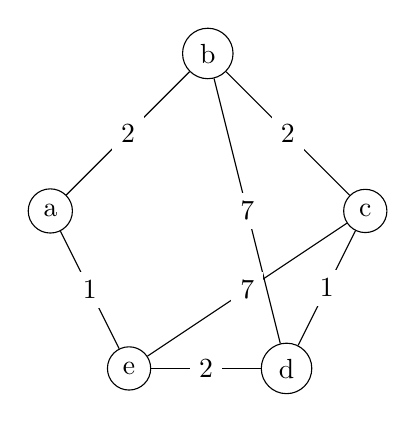
\begin{tikzpicture}[every node/.style={fill=white}, n/.style={circle, draw}]
        \node[n] (a) at (0, 0) {a};
        \node[n] (b) at (2, 2) {b};
        \node[n] (c) at (4, 0) {c};
        \node[n] (d) at (3, -2) {d};
        \node[n] (e) at (1, -2) {e};

        \draw (a) edge node {2} (b);
        \draw (a) edge node {1} (e);
        \draw (b) edge node {2} (c);
        \draw (b) edge node {7} (d);
        \draw (c) edge node {1} (d);
        \draw (c) edge node {7} (e);
        \draw (d) edge node {2} (e);
    \end{tikzpicture}
\end{example}

Árvore de enumeração:

\begin{example}
    \centering
    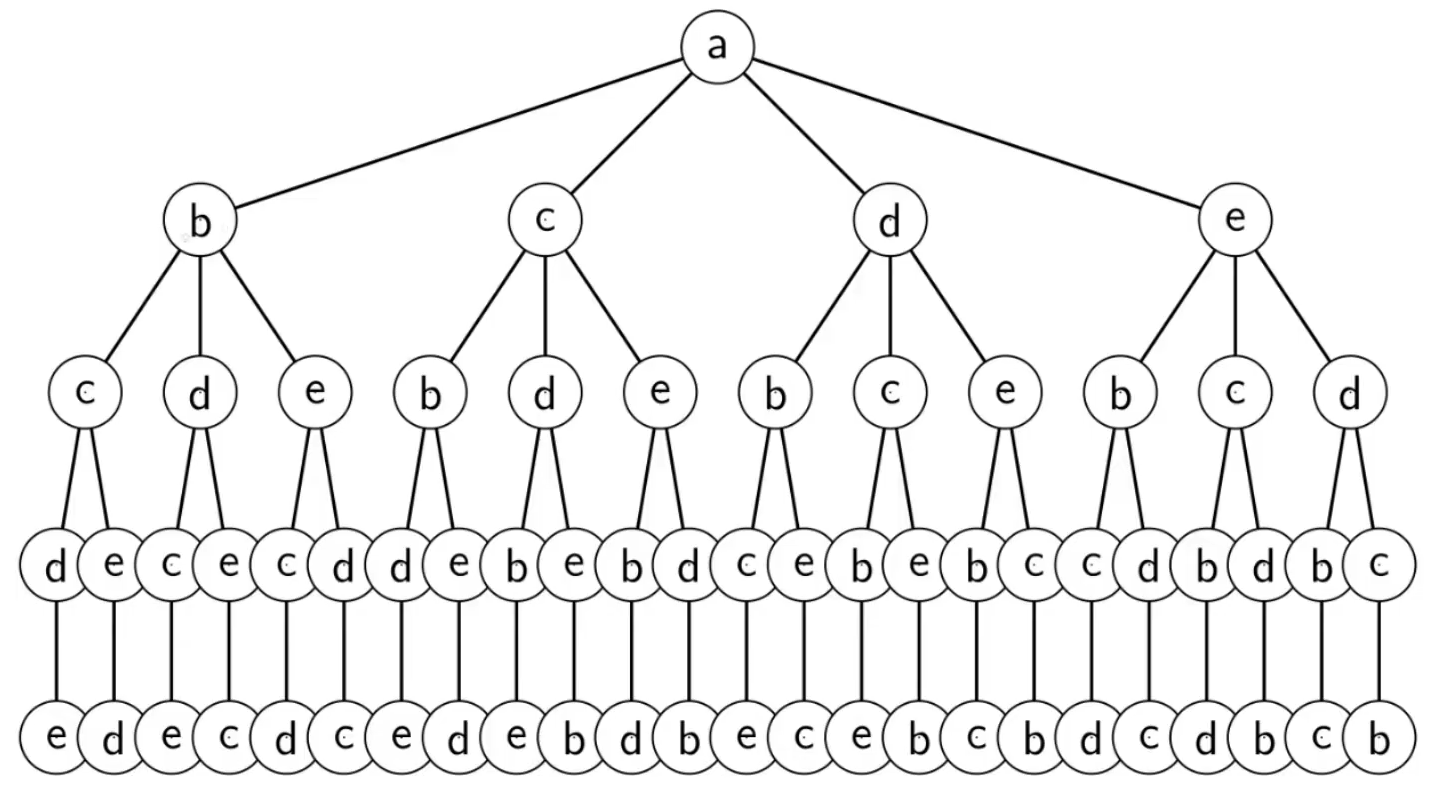
\includegraphics[width=.95\linewidth]{img/arvore_enumeracao_tsp.png}
\end{example}

Pode podar aqueles ramos que indicam um caminho impossível (sem aresta)

\begin{example}
    \centering
    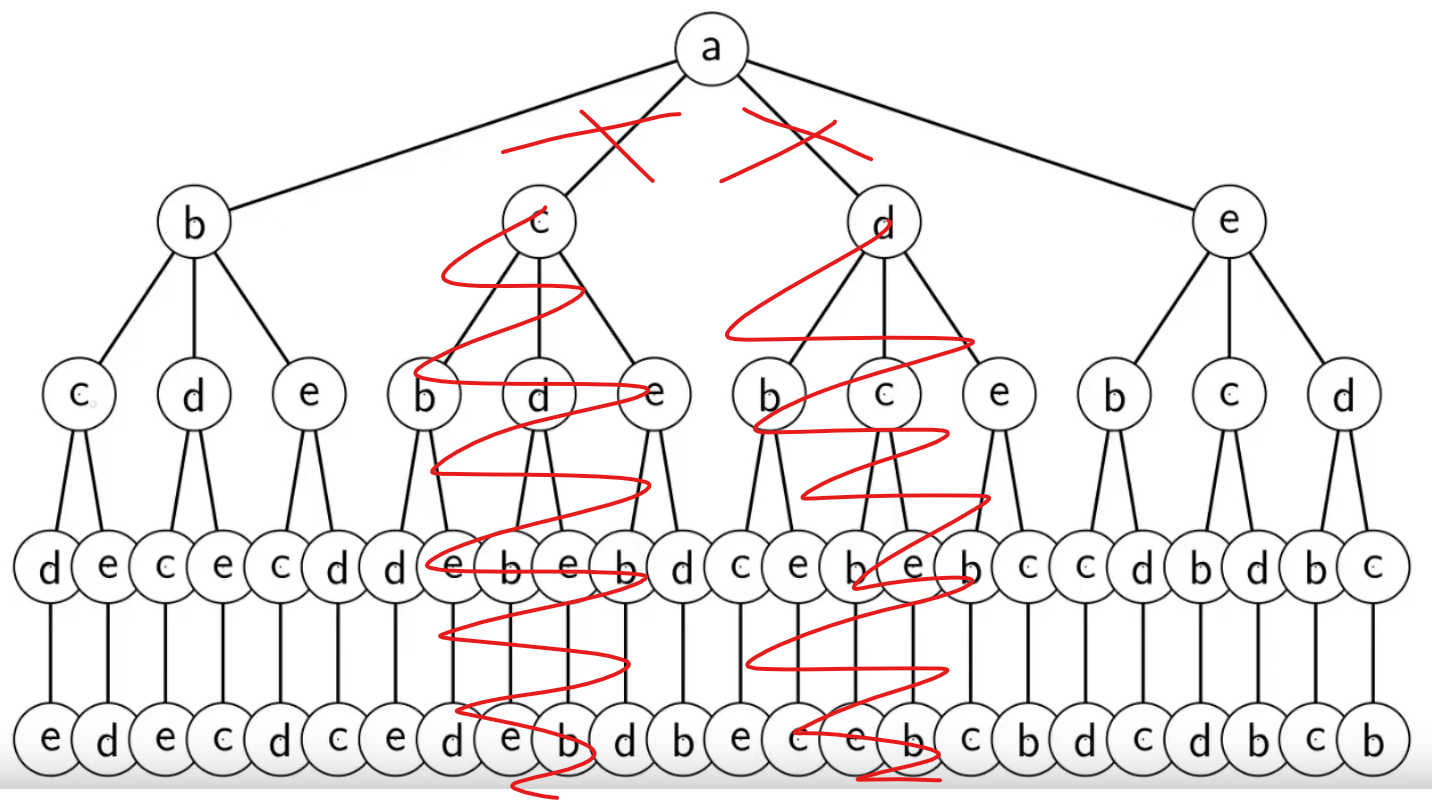
\includegraphics[width=.95\linewidth]{img/arvore_podada_tsp.png}
\end{example}

Mais podas podem ser feitas

\begin{example}
    \centering
    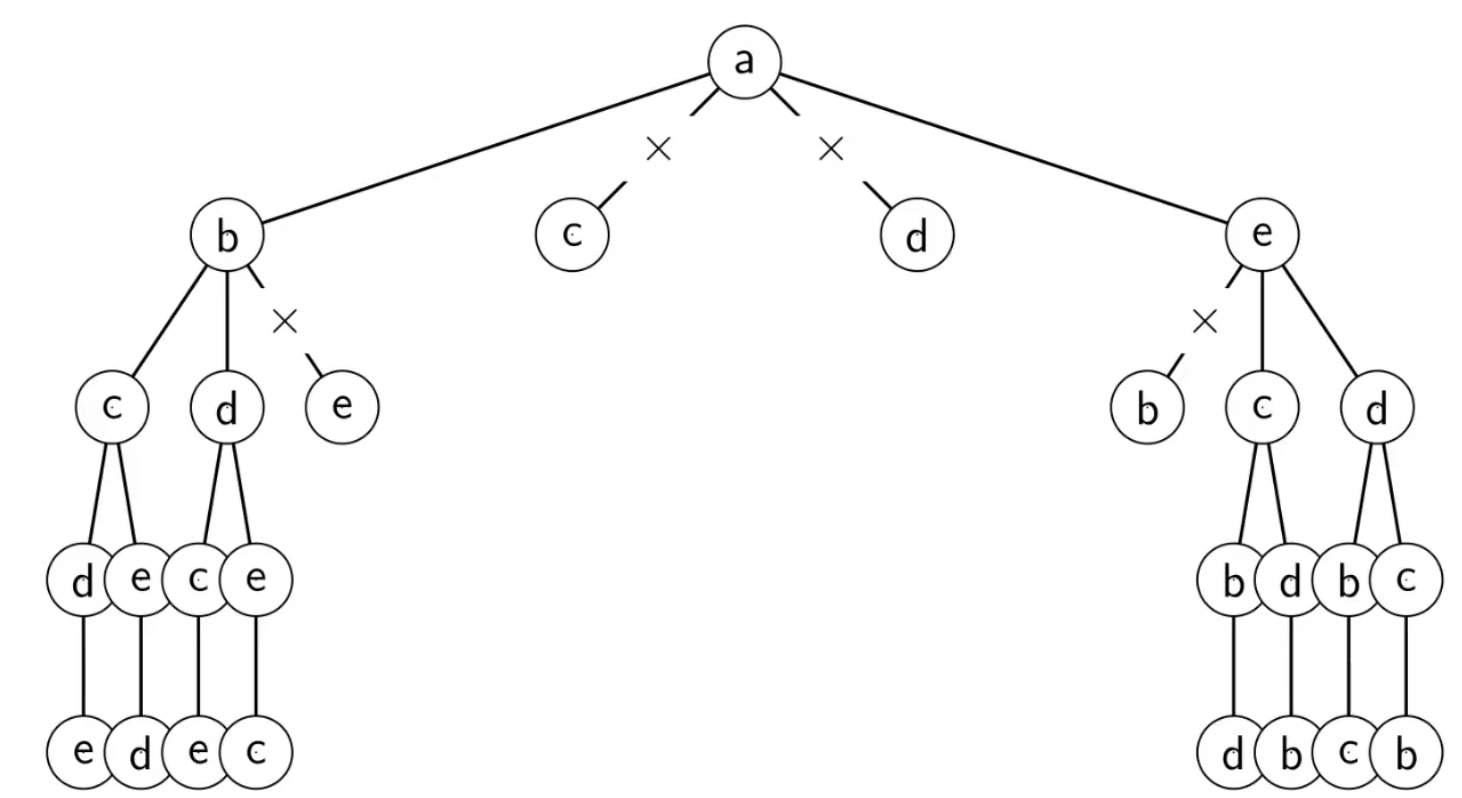
\includegraphics[width=.95\linewidth]{img/arvore_podada_tsp_2.png}
\end{example}

Levando os custos das arestas em consideração:

O caminho $a \xrightarrow{2} b \xrightarrow{2} c \xrightarrow{1} d \xrightarrow{2} e \xrightarrow{1} a$ tem custo total $8$.

O caminho $a \xrightarrow{2} b \xrightarrow{7} d$ tem custo $9$ por si só. Então tudo abaixo vai ser pior que o caminho anterior, não é promissor usar.

Com todos esses caminhos removidos, a árvore final que precisa ser percorrida fica:

\begin{example}
    \centering
    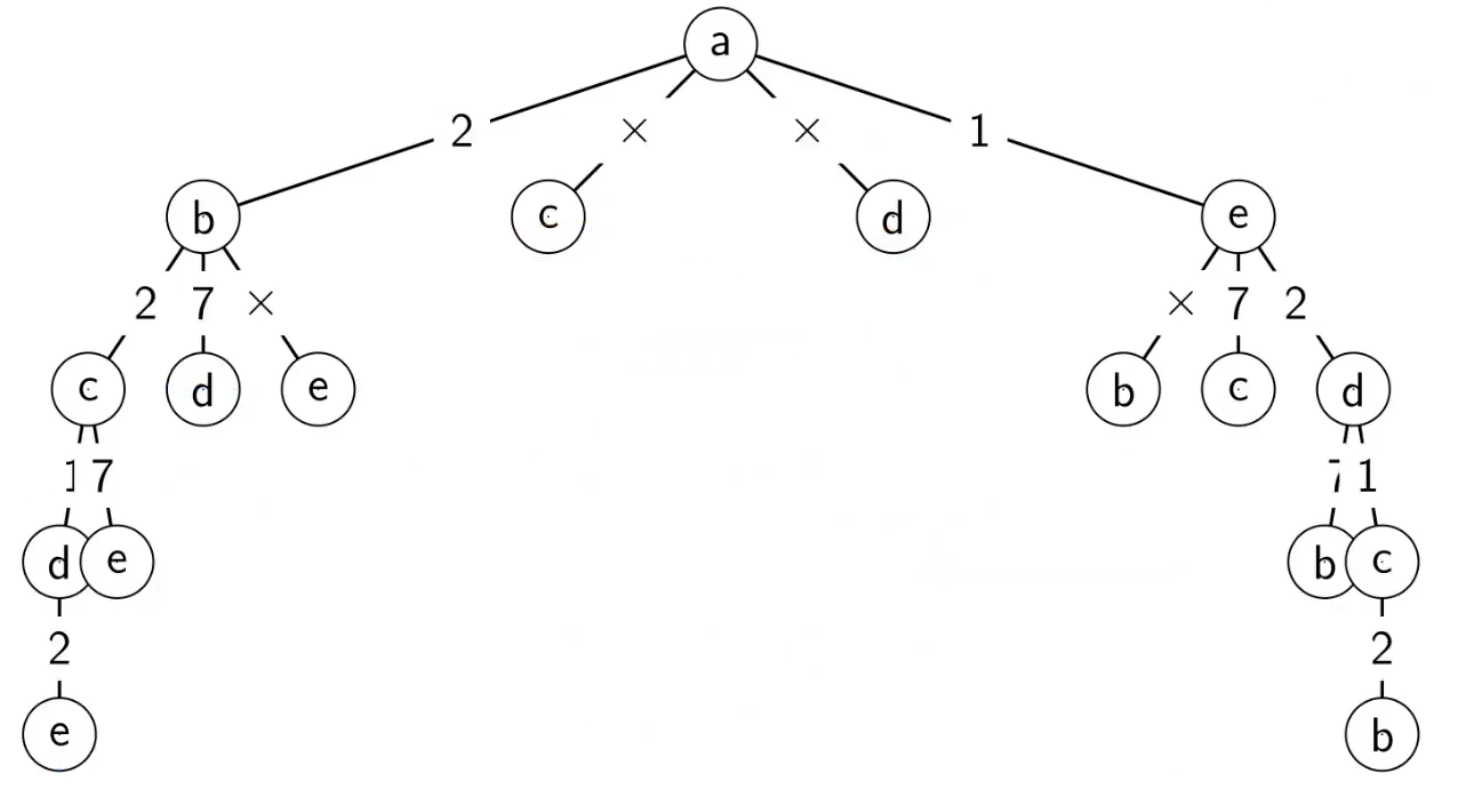
\includegraphics[width=.95\linewidth]{img/arvore_podada_tsp_final.png}
\end{example}

\subsection{Programação linear (inteira)}

Modelo matemático de otimização.

\begin{itemize}
    \item Conjunto variáveis relacionamentos
    \item Conjunto de restrições $\to$ inequações lineares
    \item Função objetivo $\to$ expressão linear
\end{itemize}

Sempre trabalhar com constantes multiplicando variáveis e soma deses valores.

Uma solução é viável se todas as restrições são atendidas.

\vspace{\baselineskip}

A forma padrão para um problema de \underline{minimização} com $n$ variáveis e $m$ restrições é:

\vspace{\baselineskip}

\begin{center}
    minimizar $\sum_{j=1}^{n}c_jx_j$

    sujeito a $\sum_{j=1}^{n}a_{ij}x_j \geq b_i \forall i \in \{1,\dots,m\}$

    $x_j \geq 0 \forall j \in \{1,\dots,n\}$
\end{center}

$a_{ij}$, $b_i$ e $c_j$ são constantes.

$x_j$ são variáveis.

Em um programa linear inteiro, as \underline{variáveis são inteiras}.

\subsubsection{Problema da Mochila}

Sejam $x_i$ variáveis binárias que indicam se o item $i$ foi ecolhido.

\begin{center}
    maximizar $\sum_{i=1}^{n}v_ix_i$

    sujeito a $\sum_{i=1}^{n}w_ix_i \leq W$

    $x_i \in \left\{ 0, 1\right\} \forall i \in \left\{ 1, \dots, n\right\}$
\end{center}

\vspace{\baselineskip}

Programas lineares podem ser resolvidos em tempo polinomial $\to$ Mochila fracionária.

Programas lineares \underline{inteiros} são, normalmente, NP-Difíceis.

Resolvedores de PLI usam o \textit{branch and bound} junto com PL.

Roda PL dentro de cada nó para encontrar limitantes inferiores para aquele ramo inteiro. Depois faz a poda.

\section{Heurísticas}

Algoritmos que encontram uma solução viável.

\textbf{Não} garante que seja solução ótima.

Tendem a ser mais rápidos.

Duas categorias:

\begin{itemize}
    \item Construtivas: Constroem uma solução viável
    \item Busca local: Partem de uma solução inicial e tentam melhorar através de modificações
\end{itemize}

\subsection{Heurística construtiva para a Mochila}

\begin{algorithm}
    \SetAlgoLined
    \SetKwFunction{Mochila}{MochilaGuloso}

    \Fn{\Mochila{$n: \mathrm{itens}$, $w: \mathrm{peso}$, $v: \mathrm{valor}$, $W: \mathrm{capacidade}$}}{
        ordene e renomeie os itens para que $\frac{v1}{w_1}\geq\frac{v_2}{w_2}\geq\dots\geq\frac{v_n}{w_n}$\;
        seja $q$ um inteiro tal que $\sum_{i=1}^{q}w_i\leq W$ e $\sum_{i=1}^{q+1} > W$\;
        \Retorna{$v_1+v_2+\dots+v_q$}
    }
\end{algorithm}

Exemplo que não funciona:

\begin{example}
    \begin{multicols}{2}
        $W=B$

        $v_1 = 2$ \quad $w_1 = 1$ \quad $\frac{v_1}{w_1}=2$

        $v_2 = B$ \quad $w_2 = B$ \quad $\frac{v_2}{w_2}=1$

        \columnbreak

        Ordem decrescetnte: 1, 2

        Fração item 1: $100\%$

        Espaço livre: $B - 1$

        Fração item 2: $0\%$
    \end{multicols}
\end{example}

A solução final é fica com valor 1 e espaço livre $B-1$. Mas a solução ótima é, claramente, pegar o item 2. Então a solução gulosa não é ótima, mas é uma solução viável.

\subsubsection{Heurística de busca local para o TSP}

Vizinhança de 2-OPT (troca de 2 arestas) de um circuito hamiltoniano $C$:

\begin{itemize}
    \item Conjunto de circuitos hamiltonianos que são obtidos removendo 2 arestas de $C$ e inserindo outras 2 arestas
\end{itemize}

Exemplo de troca 2-OPT:

\begin{example}
    \centering
    \begin{multicols}{3}
        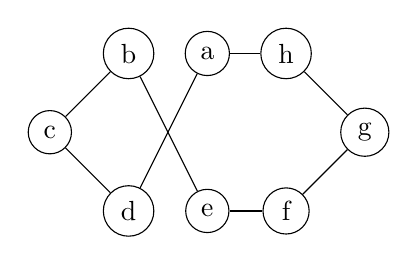
\begin{tikzpicture}[every node/.style={fill=white}, n/.style={circle, draw}]
            \node[n] (c) at (0, 0) {c};
            \node[n] (b) at (1, 1) {b};
            \node[n] (d) at (1, -1) {d};
            \node[n] (a) at (2, 1) {a};
            \node[n] (e) at (2, -1) {e};
            \node[n] (h) at (3, 1) {h};
            \node[n] (f) at (3, -1) {f};
            \node[n] (g) at (4, 0) {g};

            \draw (c) edge (b);
            \draw (b) edge (e);
            \draw (e) edge (f);
            \draw (f) edge (g);
            \draw (g) edge (h);
            \draw (h) edge (a);
            \draw (a) edge (d);
            \draw (d) edge (c);
        \end{tikzpicture}
        \columnbreak
        \vspace*{.8cm}
        {\Huge $\Rightarrow$}
        \columnbreak
        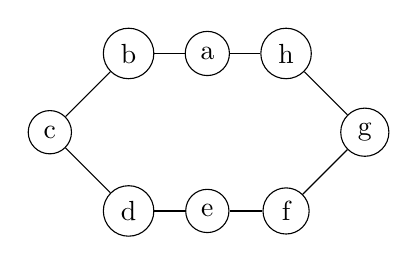
\begin{tikzpicture}[every node/.style={fill=white}, n/.style={circle, draw}]
            \node[n] (c) at (0, 0) {c};
            \node[n] (b) at (1, 1) {b};
            \node[n] (d) at (1, -1) {d};
            \node[n] (a) at (2, 1) {a};
            \node[n] (e) at (2, -1) {e};
            \node[n] (h) at (3, 1) {h};
            \node[n] (f) at (3, -1) {f};
            \node[n] (g) at (4, 0) {g};

            \draw (c) edge (b);
            \draw (b) edge (a);
            \draw (e) edge (f);
            \draw (f) edge (g);
            \draw (g) edge (h);
            \draw (h) edge (a);
            \draw (e) edge (d);
            \draw (d) edge (c);
        \end{tikzpicture}
    \end{multicols}
\end{example}

\begin{algorithm}
    \SetAlgoLined
    \SetKwFunction{TSP}{TSP-2OPT}

    \Fn{\TSP{$G=(V, E), w$}}{
        encontra um circuito hamiltoniano inicial $C$\;
        \Enqto{houver um circuito $C'$ na vizinhança 2-OPT de $C$ tal que $w(C') < w(C)$}{
            $C \gets C'$
        }
        \Retorna{C}
    }
\end{algorithm}
\chapter{Algoritmos Gulosos}

\section{Abordagens}

P $\neq$ NP $\to$ \textbf{Não} é possível encontrar um algoritmo que \underline{encontre soluções ótimas} em \underline{tempo polinomial} \underline{para qualquer entrada}.

Existem abordagens que abrem mão de alguma dessas características.

\subsection{Heurísticas}

Abre mão dee que a solução seja ótima. Encontra uma solução viável. Podem ser:

\begin{itemize}
    \item Construtivas -- Constrói uma solução viável
    \item De Busca Local -- Modifica uma solução pré-existente
\end{itemize}

\subsection{Algoritmos gulosos}

As heurísticas construtivas são normalmente estratégias gulosas.

Algoritmos gulosos tomam decisões locais de curto prazo que leve a soluções. Normalmente produz soluções ótimas para problemas específicos, mas não é garantido para problemas NP-Difíceis.

É necessário criatividade para propor métodos gulosos para um problema.

\section{Problema do Escalonamento}

\begin{itemize}
    \item \textbf{Entrada:} conjunto de tarefas $\left\{ 1,\dots,n\right\}$, cada tarefa $i$ tem tempo de processamento $t_i$ e $m$ máquinas idênticas.
    \item \textbf{Soluções viáveis:} partição das tarefas em $m$ conjuntos $M_1, M_2, \dots, M_m$.
    \item \textbf{Função objetivo:} $\max_{j=1\dots m}\sum_{i \in M_j}t_i$ (makespan).
    \item \textbf{Objetivo:} encontrar solução de custo mínimo.
\end{itemize}

\subsection{Algoritmo guloso para o escalonamento}

\begin{algorithm}
    \SetAlgoLined
    \SetKwFunction{Escalona}{EscalonaGuloso}

    \Fn{\Escalona{$n$, $t$, $m$}}{
        \lPara{$j \gets 1$ até $m$}{ $M_j=\emptyset$}
        \Para{$i \gets 1$ até $n$}{
            seja $j$ uma máquina em que $\sum_{i \in M_j}t_i$ é mínimo\;
            $M_j \gets M_j \cup \left\{i\right\}$\;
        }
        \Retorna{$\max_{j=1,\dots,m}\sum_{i \in M_j}t_i$}\;
    }
\end{algorithm}

\begin{example}
    $m=2$

    \begin{multicols}{2}

        \tikzset{tempo/.style 2 args={rectangle split, rectangle split horizontal, draw=#2, rectangle split parts=#1, fill=#2!20}}

        \begin{center}
            \begin{tikzpicture}
                \node[tempo={2}{blue}, label=below:$t_1$] (t1) at (0, 0) {};
                \node[tempo={1}{red}, label=below:$t_2$] (t2) [right=of t1] {};
                \node[tempo={1}{green}, label=below:$t_3$] (t3) [right=of t2] {};
            \end{tikzpicture}
        \end{center}

        \begin{tabular}{l|l}
            $M_1$ & \tikzmark{2m11} \\
            $M_2$ & \tikzmark{2m21} \\
        \end{tabular}

        \begin{tikzpicture}[remember picture, tempo/.append style={anchor=west, overlay}, node distance=1pt]
            \node[tempo={2}{blue}] (t1) at (pic cs:2m11) {};
            \node[tempo={1}{red}] (t2) at (pic cs:2m21) {};
            \node[tempo={1}{green}] (t3) [right=of t2] {};
        \end{tikzpicture}

        \begin{center}
            \textit{makespan} = $2$
        \end{center}

        \columnbreak

        \begin{center}
            \begin{tikzpicture}
                \node[tempo={1}{red}, label=below:$t_1$] (t1) at (0, 0) {};
                \node[tempo={1}{green}, label=below:$t_2$] (t2) [right=of t1] {};
                \node[tempo={2}{blue}, label=below:$t_3$] (t3) [right=of t2] {};
            \end{tikzpicture}
        \end{center}

        \begin{tabular}{l|l}
            $M_1$ & \tikzmark{2m12} \\
            $M_2$ & \tikzmark{2m22} \\
        \end{tabular}

        \begin{tikzpicture}[remember picture, tempo/.append style={anchor=west, overlay}, node distance=1pt]
            \node[tempo={1}{red}] (t1) at (pic cs:2m12) {};
            \node[tempo={1}{green}] (t2) at (pic cs:2m22) {};
            \node[tempo={2}{blue}] (t3) [right=of t1] {};
        \end{tikzpicture}

        \begin{center}
            \textit{makespan} = $3$
        \end{center}
    \end{multicols}
\end{example}

A ordem nos trabalhos mudou e o algoritmo não encontrou a solução ótima. A ideia é lidar primeiro com os trabalhos mais longos.

\begin{algorithm}
    \SetAlgoLined
    \SetKwFunction{Escalona}{EscalonaGuloso2}
    \Fn{\Escalona{$n$, $t$, $m$}}{
        \lPara{$j \gets 1$ até $m$}{ $M_j=\emptyset$}
        \underline{Ordene e renomeie os itens de modo que $t_1 \geq t_2 \geq \dots \geq t_n$}\;
        \Para{$i \gets 1$ até $n$}{
            seja $j$ uma máquina em que $\sum_{i \in M_j}t_i$ é mínimo\;
            $M_j \gets M_j \cup \left\{i\right\}$\;
        }
        \Retorna{$\max_{j=1,\dots,m}\sum_{i \in M_j}t_i$}\;
    }
\end{algorithm}

Neste caso, ordenar ainda não gera a solução ótima. Não ordenar ainda gera um makespan menor:

\begin{example}
    $m=2$

    \tikzset{tempo/.style 2 args={rectangle split, rectangle split horizontal, draw=#2, rectangle split parts=#1, fill=#2!20}}

    \begin{center}
        \begin{tikzpicture}[node distance=.25cm]
            \node[tempo={3}{orange}] (t1) at (0, 0) {};
            \node[tempo={2}{blue}] (t2) [right=of t1] {};
            \node[tempo={2}{red}] (t3) [right=of t2] {};
            \node[tempo={3}{green}] (t4) [right=of t3] {};
            \node[tempo={2}{violet}] (t5) [right=of t4] {};
        \end{tikzpicture}
    \end{center}

    \begin{multicols}{2}
        Ordenando:

        \begin{tikzpicture}[node distance=.25cm]
            \node[tempo={3}{orange}] (t1) at (0, 0) {};
            \node[tempo={3}{green}] (t2) [right=of t1] {};
            \node[tempo={2}{blue}] (t3) [right=of t2] {};
            \node[tempo={2}{red}] (t4) [right=of t3] {};
            \node[tempo={2}{violet}] (t5) [right=of t4] {};
        \end{tikzpicture}

        \vspace{\baselineskip}

        \begin{tabular}{l|l}
            $M_1$ & \tikzmark{3m11} \\
            $M_2$ & \tikzmark{3m21} \\
        \end{tabular}

        \begin{tikzpicture}[remember picture, , tempo/.append style={anchor=west, overlay}, node distance=1pt]
            \node[tempo={3}{orange}] (t1) at (pic cs:3m11) {};
            \node[tempo={3}{green}] (t2) at (pic cs:3m21) {};
            \node[tempo={2}{blue}] (t3) [right=of t1] {};
            \node[tempo={2}{red}] (t4) [right=of t2] {};
            \node[tempo={2}{violet}] (t5) [right=of t3] {};
        \end{tikzpicture}

        \begin{center}
            \textit{makespan} = $7$
        \end{center}

        \columnbreak

        Sem ordenar:

        \vspace{\baselineskip}
        \vspace{\baselineskip}

        \begin{tabular}{l|l}
            $M_1$ & \tikzmark{3m12} \\
            $M_2$ & \tikzmark{3m22} \\
        \end{tabular}

        \begin{tikzpicture}[remember picture, , tempo/.append style={anchor=west, overlay}, node distance=1pt]
            \node[tempo={3}{orange}] (t1) at (pic cs:3m12) {};
            \node[tempo={2}{blue}] (t2) at (pic cs:3m22) {};
            \node[tempo={2}{red}] (t3) [right=of t2] {};
            \node[tempo={3}{green}] (t4) [right=of t1] {};
            \node[tempo={2}{violet}] (t5) [right=of t3] {};
        \end{tikzpicture}

        \begin{center}
            \textit{makespan} = $6$
        \end{center}
    \end{multicols}
\end{example}

Como estamos lidando com heurísticas, quase sempre é possível indicar um caso que o algoritmo mais simples funciona melhor que o mais sofisticado. Mas ordenar ainda é melhor \underline{em geral}.

Lidando com problemas NP-Difíceis. O ideal é executar diferentes métodos e selecionar o melhor resultado. Variedade é importante, principalmente se os diversos métodos já são velozes.

\section{Problema da Mochila}

\begin{itemize}
    \item \textbf{Entrada:} conjunto de $n$ itens, cada item $i$ tem peso $w_i$ e valor $v_i$ e tamanho $W$ da mochila.
    \item \textbf{Soluções viáveis:} conjuntos de itens $S \subseteq \left\{1,\dots,n\right\}$ com $\sum_{i \in S}w_i \leq W$.
    \item \textbf{Função objetivo:} soma dos valores dos itens em $S$.
    \item \textbf{Objetivo:} encontrar uma solução de valor máximo.
\end{itemize}

\begin{algorithm}
    \SetAlgoLined
    \SetKwFunction{Mochila}{MochilaGuloso}

    \Fn{\Mochila{$n$, $w$, $v$, $W$}}{
        $S \gets \emptyset$ \tcc*{Solução}
        $R \gets W$ \tcc*{Espaço restante}
        Ordene e renomeie os itens para que $\frac{v_1}{w_1}\geq\frac{v_2}{w_2}\geq\dots\geq\frac{v_n}{w_n}$
        \Para{$i \gets 1$ até $n$}{
            \Se(\tcc*[f]{Se couber na mochila}){$w_i \leq R$}{
                $S \gets S \cup \left\{ i \right\}$ \tcc*{Adicione $i$ à mochila}
                $R \gets R - w_i$
            }
        }
        \Retorna S
    }
\end{algorithm}

\begin{example}
    \tikzset{item/.style 2 args={rectangle split, rectangle split horizontal, draw=#2, rectangle split parts=#1, fill=#2!20}}

    \begin{center}
        \begin{tikzpicture}
            \node[item={2}{blue}] (1) at (0, 0) {};
            \node[align=center, anchor=north] (l1) at (1.south) {$w_1 = 2$\\$v_1 = 3$\\$\frac{v_1}{w_1}=\frac{3}{2}$};
            \node [below right=-.75cm and 0cm of l1] {\large $>$};
            \node[item={3}{green}] (2) [right=of 1] {};
            \node[align=center, anchor=north] (l2) at (2.south) {$w_2 = 3$\\$v_1 = 4$\\$\frac{v_2}{w_2}=\frac{4}{3}$};
            \node [below right=-.75cm and .25cm of l2] {\large $>$};
            \node[item={4}{orange}] (3) [right=of 2] {};
            \node[align=center, anchor=north] (l3) at (3.south) {$w_3 = 4$\\$v_3 = 5$\\$\frac{v_3}{w_3}=\frac{5}{4}$};
        \end{tikzpicture}

        \vspace{\baselineskip}

        Algoritmo guloso baseado na razão $\frac{\mathrm{valor}}{\mathrm{peso}}$
    \end{center}

    \begin{multicols}{3}
        \begin{center}
            $W = 5$

            \begin{tikzpicture}[item/.append style={anchor=west}, node distance=1pt]
                \node[item={2}{blue}] (1) at (0, 0) {};
                \node[item={3}{green}] (2) [right=of 1] {};
            \end{tikzpicture}

            Solução = 7
        \end{center}

        \columnbreak

        \begin{center}
            $W = 6$

            \begin{tikzpicture}[item/.append style={anchor=west}, node distance=1pt]
                \node[item={2}{blue}] (1) at (0, 0) {};
                \node[item={3}{green}] (2) [right=of 1] {};
            \end{tikzpicture}

            Solução = 7
        \end{center}

        \columnbreak

        \begin{center}
            $W = 4$

            \begin{tikzpicture}[item/.append style={anchor=west}, node distance=1pt]
                \node[item={2}{blue}] (1) at (0, 0) {};
            \end{tikzpicture}

            Solução = 3
        \end{center}
    \end{multicols}

    \begin{center}
        Solução ótima
    \end{center}

    \begin{multicols}{3}
        \begin{center}
            $W = 5$

            \begin{tikzpicture}[item/.append style={anchor=west}, node distance=1pt]
                \node[item={2}{blue}] (1) at (0, 0) {};
                \node[item={3}{green}] (2) [right=of 1] {};
            \end{tikzpicture}

            Solução = 7
        \end{center}

        \columnbreak

        \begin{center}
            $W = 6$

            \begin{tikzpicture}[item/.append style={anchor=west}, node distance=1pt]
                \node[item={2}{blue}] (1) at (0, 0) {};
                \node[item={4}{orange}] (2) [right=of 1] {};
            \end{tikzpicture}

            Solução = 8
        \end{center}

        \columnbreak

        \begin{center}
            $W = 4$

            \begin{tikzpicture}[item/.append style={anchor=west}, node distance=1pt]
                \node[item={4}{orange}] (1) at (0, 0) {};
            \end{tikzpicture}

            Solução = 5
        \end{center}
    \end{multicols}

    \begin{center}
        Algoritmo guloso baseado no valor
    \end{center}

    \begin{multicols}{3}
        \begin{center}
            $W = 5$

            \begin{tikzpicture}[item/.append style={anchor=west}, node distance=1pt]
                \node[item={4}{orange}] (1) at (0, 0) {};
            \end{tikzpicture}

            Solução = 5
        \end{center}

        \columnbreak

        \begin{center}
            $W = 6$

            \begin{tikzpicture}[item/.append style={anchor=west}, node distance=1pt]
                \node[item={4}{orange}] (1) at (0, 0) {};
                \node[item={2}{blue}] (2) [right=of 1] {};
            \end{tikzpicture}

            Solução = 8
        \end{center}

        \columnbreak

        \begin{center}
            $W = 4$

            \begin{tikzpicture}[item/.append style={anchor=west}, node distance=1pt]
                \node[item={4}{orange}] (1) at (0, 0) {};
            \end{tikzpicture}

            Solução = 5
        \end{center}
    \end{multicols}
\end{example}

\begin{algorithm}
    \SetAlgoLined
    \SetKwFunction{Mochila}{MochilaGuloso2}

    \Fn{\Mochila{$n, w, v, W$}}{
        $S \gets \emptyset$ \tcc*{Solução}
        $R \gets W$ \tcc*{Espaço restante}
        Ordene e renomeie os itens para que $v_1 \geq v_2 \geq \dots \geq v_n$
        \Para{$i \gets 1$ até $n$}{
            \Se(\tcc*[f]{Se couber na mochila}){$w_i \leq R$}{
                $S \gets S \cup \left\{ i \right\}$ \tcc*{Adicione $i$ à mochila}
                $R \gets R - w_i$
            }
        }
        \Retorna S
    }
\end{algorithm}

O algoritmo guloso baseado em razão se deu melhor em uma instância e o baseado em valor foi melhor em duas intâncias. $\implies$ O melhor é \underline{combinar os algoritmos}.

\section{Problema da Coloração}

\begin{itemize}
    \item \textbf{Entrada:} um grafo $G = (V, E)$.
    \item \textbf{Soluções viáveis:} partição $V_1, V_2, \dots , V_q$ de $V$ tal que toda aresta $(u, v) \in E$ tem extremos em partes distintas.
    \item \textbf{Função objetivo:} número $q$ te partes (cores) utilizadas.
    \item \textbf{Objetivo:} encontrar solução de custo mínimo.
\end{itemize}

\begin{algorithm}
    \SetAlgoLined
    \SetKwFunction{Coloracao}{ColoracaoGuloso}

    \Fn{\Coloracao{$G=(V, E)$}}{
        \Para{$v \in V$}{
            \tcc{Cores representadas por índices em ordem}
            seja $i$ a menor cor não presente nos vizinhos de $v$\;
            atribua cor $i$ a $v$\;
        }
        seja $i_{\mathrm{max}}$ a maior cor utilizada\;
        \Retorna $i_{\mathrm{max}}$
    }
\end{algorithm}

\begin{example}
    \begin{center}
        Grafo de Petersen

        Cores: \textcolor{orange}{1} \textcolor{blue}{2} \textcolor{green}{3} \textcolor{violet}{4}

        \vspace{\baselineskip}

        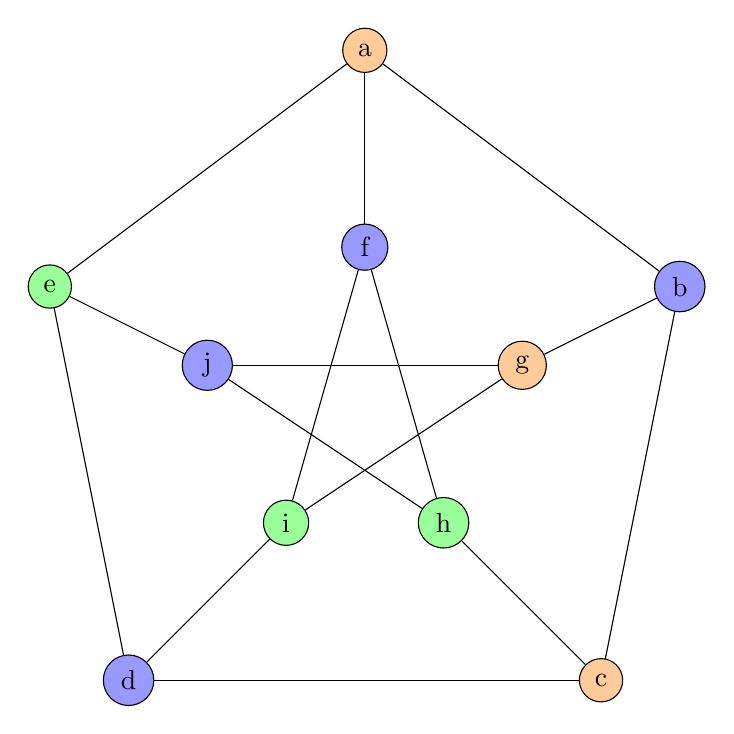
\begin{tikzpicture}[every node/.style={fill=white}, n/.style={circle, draw, fill=#1!40}]
            \node[n={orange}] (a) at (1, 4) {a};
            \node[n={blue}] (b) at (5, 1) {b};
            \node[n={orange}] (c) at (4, -4) {c};
            \node[n={blue}] (d) at (-2, -4) {d};
            \node[n={green}] (e) at (-3, 1) {e};
            \node[n={blue}] (f) at (1, 1.5) {f};
            \node[n={orange}] (g) at (3, 0) {g};
            \node[n={green}] (h) at (2, -2) {h};
            \node[n={green}] (i) at (0, -2) {i};
            \node[n={blue}] (j) at (-1, 0) {j};

            \draw (a) edge (b);
            \draw (a) edge (f);
            \draw (a) edge (e);
            \draw (b) edge (g);
            \draw (b) edge (c);
            \draw (c) edge (h);
            \draw (c) edge (d);
            \draw (d) edge (i);
            \draw (d) edge (e);
            \draw (e) edge (j);
            \draw (f) edge (h);
            \draw (f) edge (i);
            \draw (g) edge (i);
            \draw (g) edge (j);
            \draw (h) edge (j);
        \end{tikzpicture}

        Resultado: 3 cores
    \end{center}
\end{example}

\begin{example}
    \centering
    Cores: \textcolor{orange}{1} \textcolor{blue}{2} \textcolor{green}{3} \textcolor{violet}{4}

    \vspace{\baselineskip}

    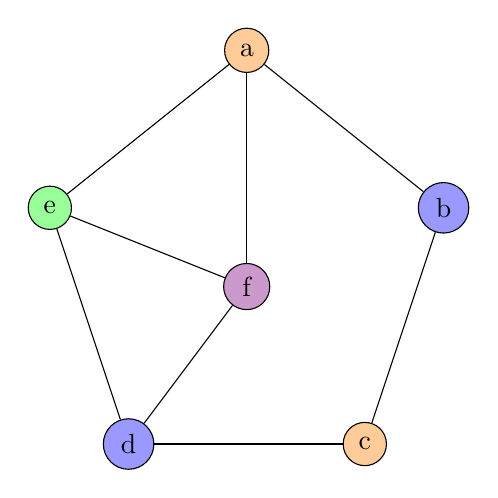
\begin{tikzpicture}[every node/.style={fill=white}, n/.style={circle, draw, fill=#1!40}]
        \node[n={orange}] (a) at (0.5, 2) {a};
        \node[n={blue}] (b) at (3, 0) {b};
        \node[n={orange}] (c) at (2, -3) {c};
        \node[n={blue}] (d) at (-1, -3) {d};
        \node[n={green}] (e) at (-2, 0) {e};
        \node[n={violet}] (f) at (0.5, -1) {f};

        \draw (a) edge (b);
        \draw (a) edge (e);
        \draw (a) edge (f);
        \draw (b) edge (c);
        \draw (c) edge (d);
        \draw (d) edge (e);
        \draw (d) edge (f);
        \draw (e) edge (f);
    \end{tikzpicture}

    Resultado: 4 cores
\end{example}

O problema aqui foi um vértice de maior grau (f). Uma ideia é começar a trabalhar com os vértices de maior grau.

Reordenando, temos:

\begin{example}
    \centering
    Cores: \textcolor{orange}{1} \textcolor{blue}{2} \textcolor{green}{3} \textcolor{violet}{4}

    \vspace{\baselineskip}

    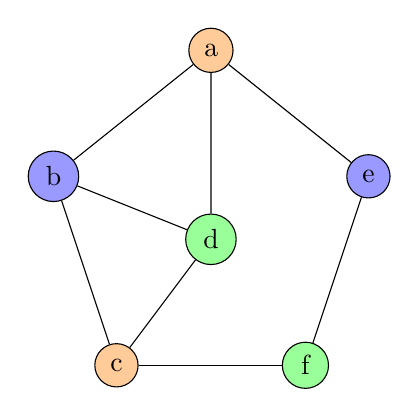
\begin{tikzpicture}[every node/.style={fill=white}, n/.style={circle, draw, fill=#1!40}, scale=.8]
        \node[n={orange}] (a) at (0.5, 2) {a};
        \node[n={blue}] (e) at (3, 0) {e};
        \node[n={green}] (f) at (2, -3) {f};
        \node[n={orange}] (c) at (-1, -3) {c};
        \node[n={blue}] (b) at (-2, 0) {b};
        \node[n={green}] (d) at (0.5, -1) {d};

        \draw (a) edge (b);
        \draw (a) edge (d);
        \draw (a) edge (e);
        \draw (b) edge (c);
        \draw (b) edge (d);
        \draw (c) edge (d);
        \draw (c) edge (f);
        \draw (e) edge (f);
    \end{tikzpicture}

    Resultado: 4 cores
\end{example}

\begin{algorithm}
    \SetAlgoLined
    \SetKwFunction{Coloracao}{ColoracaoGuloso2}
    \Fn{\Coloracao{$G=(V, E)$}}{
        ordene e renomeie os vértices em ordem decrescente de grau\;
        \Para{$v \gets 1$ até $|V|$}{
            seja $i$ a menor cor não presente nos vizinhos de $v$\;
            atribua a cor $i$ a $v$\;
        }
        seja $i_{\mathrm{max}}$ a maior cor utilizazda\;
        \Retorna $i_{\mathrm{max}}$
    }
\end{algorithm}

\section{Corte em grafos}

Um corte é uma bipartição dos vértices de um grafo.

O tamanho do corte é o número de arestas que ``atravessam'' o corte.

\begin{center}
    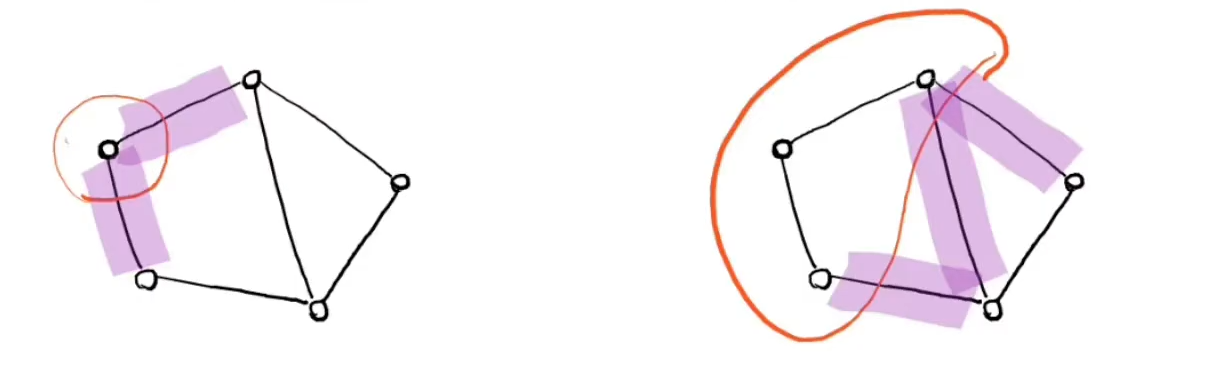
\includegraphics[width=.8\textwidth]{img/arestas_corte.png}
\end{center}

\subsection{Problema do corte máximo}

\begin{itemize}
    \item \textbf{Entrada:} um grafo $G=(V, E)$.
    \item \textbf{Soluções viáveis:} um corte de G, i.e., um conjunto $S$ tal que $\emptyset \neq S \subset V$.
    \item \textbf{Função objetivo:} número de arestas que sai de $S$: $|\delta (S)|$.
    \item \textbf{Objetivo:} encontrar solução de custo máximo.
\end{itemize}

\begin{algorithm}
    \SetAlgoLined
    \SetKwFunction{Corte}{CorteMaximoGuloso}
    \Fn{\Corte{$G=(V, E)$}}{
        $S \gets \emptyset$\;
        $\bar{S} \gets \emptyset$\;
        \Para{$v \in V$}{
            \tcc{Coloca o vértice no conjunto que tem menos vizinhos dele (aumentando o número de arestas que atravessam o corte)}
            \eSe{$|\left\{ (v, u) \in \delta(v): u \in S\right\}| \leq |\left\{ (v, u) \in \delta(v): u \in \bar{S}\right\}|$}{
                $S \gets S \cup {v}$\;
            }{
                $\bar{S} \gets \bar{S}\cup\left\{v\right\}$
            }
        }
    }
\end{algorithm}

\begin{example}
    \centering
    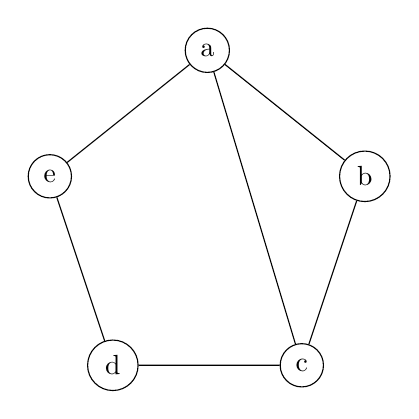
\begin{tikzpicture}[every node/.style={fill=white}, n/.style={circle, draw}, scale=.8]
        \node[n] (a) at (0.5, 2) {a};
        \node[n] (b) at (3, 0) {b};
        \node[n] (c) at (2, -3) {c};
        \node[n] (d) at (-1, -3) {d};
        \node[n] (e) at (-2, 0) {e};

        \draw (a) edge (b);
        \draw (a) edge (c);
        \draw (b) edge (c);
        \draw (c) edge (d);
        \draw (d) edge (e);
        \draw (e) edge (a);
    \end{tikzpicture}

    \vspace{\baselineskip}

    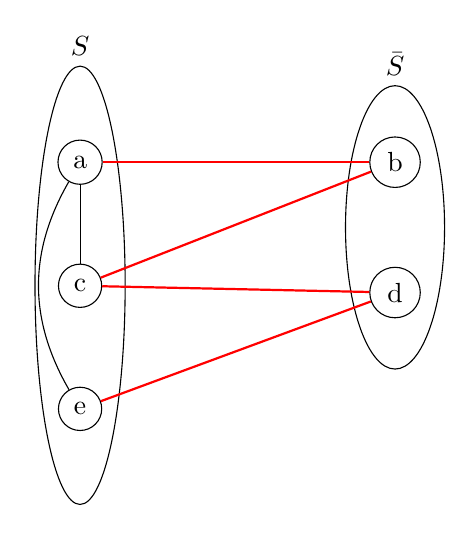
\begin{tikzpicture}[every node/.style={fill=white}, n/.style={circle, draw}]
        \node[n] (a) at (0, 0) {a};
        \node[n] (c) [below=of a] {c};
        \node[n] (e) [below=of c] {e};
        \node[n] (b) at (4, 0) {b};
        \node[n] (d) [below=of b] {d};

        \node[fill=none, draw, ellipse, fit=(a)(c)(e), label=above:$S$] {};
        \node[fill=none, draw, ellipse, fit=(b)(d), label=above:$\bar{S}$] {};

        \draw[thick, red] (a) edge (b);
        \draw (a) edge (c);
        \draw[thick, red] (b) edge (c);
        \draw[thick, red] (c) edge (d);
        \draw[thick, red] (d) edge (e);
        \draw (e) to[out=120, in=-120] (a);
    \end{tikzpicture}

    Solução: 4 arestas
\end{example}

Se atribuir mais cedo os vértices de maior grau (a, c), parece que é melhor. Já que esses vértices ``influenciam mais'' outros.

\begin{example}
    \centering
    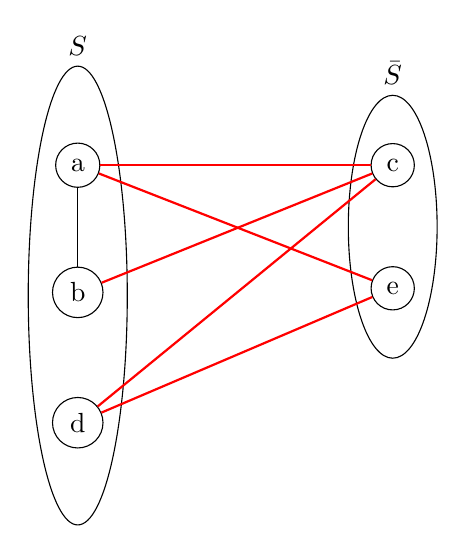
\begin{tikzpicture}[every node/.style={fill=white}, n/.style={circle, draw}]
        \node[n] (a) at (0, 0) {a};
        \node[n] (c) at (4, 0) {c};
        \node[n] (b) [below=of a] {b};
        \node[n] (d) [below=of b] {d};
        \node[n] (e) [below=of c] {e};

        \node[fill=none, draw, ellipse, fit=(a)(b)(d), label=above:$S$] {};
        \node[fill=none, draw, ellipse, fit=(c)(e), label=above:$\bar{S}$] {};

        \draw (a) edge (b);
        \draw[thick, red] (a) edge (c);
        \draw[thick, red] (b) edge (c);
        \draw[thick, red] (c) edge (d);
        \draw[thick, red] (d) edge (e);
        \draw[thick, red] (e) edge (a);
    \end{tikzpicture}

    Solução: 5 arestas
\end{example}

\begin{algorithm}
    \SetAlgoLined
    \SetKwFunction{Corte}{CorteMaximoGuloso2}
    \Fn{\Corte{$G=(V, E)$}}{
        $S \gets \emptyset$\;
        $S \gets \emptyset$\;
        $alcancados \gets \left\{ s \right\}$ \tcc*{Inicializa com algum vértice inicial}
        \Para{$v \in alcancados$ \underline{com maior grau}}{
            \eSe{$|\left\{ (v, u) \in \delta(v): u \in S\right\}| \leq |\left\{ (v, u) \in \delta(v): u \in \bar{S}\right\}|$}{
                $S \gets S \cup {v}$\;
                $alcancados \gets alcancados \cup \delta(v)$\;
            }{
                $\bar{S} \gets \bar{S}\cup\left\{v\right\}$\;
                $alcancados \gets alcancados \cup \delta(v)$\;
            }
        }
    }
\end{algorithm}

\section{Problema do Caixeiro Viajante}

\begin{itemize}
    \item \textbf{Entrada:} $G=(V,E)$ e função $\mathrm{w}$ de peso nas arestas.
    \item \textbf{Soluções viáveis:} circuitos hamiltonianos (visitam todos os vértices sem repetição) de $G$.
    \item \textbf{Função objetivo:} soma dos pesos das arestas do circuito.
    \item \textbf{Objetivo:} encontrar um circuito de menor custo.
\end{itemize}

Escolher em cada iteração o vértice com menor custo.

\begin{algorithm}
    \SetAlgoLined
    \SetKwFunction{TSPum}{TSP-Guloso1}
    \Fn{\TSPum{$G=(V, E), \mathrm{w}$}}{
        Seja $C$ um circuito trivial\;
        \Enqto{C não é hamiltoniano}{
            escolha uma aresta $(u, v) \in C$ e um vértice $x \notin C$ que minimizem $\mathrm{w}(u,x) + \mathrm{w}(x,v) - \mathrm{w}(u,v)$\;
            $C \gets C - uv + ux + xv$\;
        }
        \Retorna C
    }
\end{algorithm}

\newpage

\begin{example}
    \begin{center}
        \begin{tikzpicture}[every node/.style={fill=white}, n/.style={circle, draw}]
            \node[n] (a) at (4, 5) {a};
            \node[n] (b) at (0, 0) {b};
            \node[n] (c) at (3, 2) {c};
            \node[n] (d) at (7, 3) {d};
            \node[n] (e) at (5, 0) {e};
            \node[n] (f) at (0, 3) {f};
            \node[n] (g) at (2, -2) {g};

            \draw (a) edge (b);
            \draw (b) edge (c);
            \draw (c) edge (a);
            \draw[dashed] (c) edge (g);
            \draw[dashed] (b) edge (g);
        \end{tikzpicture}
    \end{center}

    Circuito trivial: $\bar{abc}$.

    Vértice que minimiza: $g$, quando inserido entre $b$ e $c$.

    Então, remove a aresta $\bar{bc}$ e adiciona $\bar{bgc}$.

    \begin{center}
        \begin{tikzpicture}[every node/.style={fill=white}, n/.style={circle, draw}]
            \node[n] (a) at (4, 5) {a};
            \node[n] (b) at (0, 0) {b};
            \node[n] (c) at (3, 2) {c};
            \node[n] (d) at (7, 3) {d};
            \node[n] (e) at (5, 0) {e};
            \node[n] (f) at (0, 3) {f};
            \node[n] (g) at (2, -2) {g};

            \draw (a) edge (b);
            \draw (c) edge (a);
            \draw (c) edge (g);
            \draw (b) edge (g);
            \draw[dashed] (g) edge (e);
            \draw[dashed] (e) edge (c);
        \end{tikzpicture}
    \end{center}

    \newpage

    Em seguida, insere o vértice $f$.

    \begin{center}
        \begin{tikzpicture}[every node/.style={fill=white}, n/.style={circle, draw}]
            \node[n] (a) at (4, 5) {a};
            \node[n] (b) at (0, 0) {b};
            \node[n] (c) at (3, 2) {c};
            \node[n] (d) at (7, 3) {d};
            \node[n] (e) at (5, 0) {e};
            \node[n] (f) at (0, 3) {f};
            \node[n] (g) at (2, -2) {g};

            \draw (a) edge (b);
            \draw (c) edge (a);
            \draw (b) edge (g);
            \draw (g) edge (e);
            \draw (e) edge (c);
            \draw[dashed] (f) edge (a);
            \draw[dashed] (f) edge (b);
        \end{tikzpicture}
    \end{center}

    E o vértice $d$ por último.

    \begin{center}
        \begin{tikzpicture}[every node/.style={fill=white}, n/.style={circle, draw}]
            \node[n] (a) at (4, 5) {a};
            \node[n] (b) at (0, 0) {b};
            \node[n] (c) at (3, 2) {c};
            \node[n] (d) at (7, 3) {d};
            \node[n] (e) at (5, 0) {e};
            \node[n] (f) at (0, 3) {f};
            \node[n] (g) at (2, -2) {g};

            \draw (c) edge (a);
            \draw (b) edge (g);
            \draw (g) edge (e);
            \draw (e) edge (c);
            \draw (f) edge (a);
            \draw (f) edge (b);
            \draw[dashed] (a) edge (d);
            \draw[dashed] (d) edge (c);
        \end{tikzpicture}
    \end{center}
\end{example}

\newpage

\subsection{Vértices mais próximos e mais distantes}

Seja $\mathrm{w}(v, C)$ a menor distância de $v$ a um vértice de $C$.

\begin{algorithm}
    \SetAlgoLined
    \SetKwFunction{TSPdois}{TSP-Guloso2}
    \Fn{\TSPdois{$G=(V, E), \mathrm{w}$}}{
        Seja $C$ um circuito trivial\;
        \Enqto{C não é hamiltoniano}{
            escolha um vértice $c \notin C$ que \underline{minimiza} $\mathrm{w}(x, C)$\;
            insira $x$ em C ao lado do vértice mais próximo dele\;
        }
        \Retorna C
    }
\end{algorithm}

É mais fácil calcular a distância de um nó para um conjunto de nós do que calcular o critério de peso de arestas do algoritmo \TSPum.

Para o algoritmo que insere o nó mais distante:

\begin{algorithm}
    \SetAlgoLined
    \SetKwFunction{TSPtres}{TSP-Guloso3}
    \Fn{\TSPtres{$G=(V, E), \mathrm{w}$}}{
        Seja $C$ um circuito trivial, de preferência formado pelos dois vértices mais distantes\;
        \Enqto{C não é hamiltoniano}{
            escolha um vértice $c \notin C$ que \underline{maximiza} $\mathrm{w}(x, C)$\;
            insira $x$ em C ao lado do vértice mais próximo dele\;
        }
        \Retorna C
    }
\end{algorithm}

Esse algoritmo não necessariamente se preocupa em adicionar as arestas de menor peso. Mas é uma heurística e gera uma solução viável.

\subsection{Vizinho mais próximo}

Não mantém um circuito. Constroi um caminho. Ao final cria um circuito ligando as extremidades.

\begin{algorithm}
    \SetAlgoLined
    \SetKwFunction{TSPquatro}{TSP-Guloso4}
    \Fn{\TSPquatro{$G=(V, E), \mathrm{w}$}}{
        Seja $v$ um vértice qualquer\;
        $C \gets (v)$\;
        \Enqto{C não contém todos os vértices}{
            Seja $C = (v_1, \dots , v_i)$\;
            Escolha um vértice $x \notin C$ que \underline{minimiza} $\mathrm{w}(v_i, x)$\;
            Insira $x$ no final de $C$\;
        }
        \Retorna C
    }
\end{algorithm}

O algoritmo \TSPquatro é mais eficiente porque não precisa calcular a distância de cada vértice ao conjunto de vértices (circuito). Calcula apenas a distância com relação a um único vértice $v_i$.
\chapter{Herísticas de busca local}
\label{chp:semana3}

Heurísticas geram soluções viáveis, mas sem garantir a qualidade.

\begin{itemize}
    \item Construtivas
    \item De busca local
\end{itemize}

\section{Introdução}

\subsection{Ótimo local vs. ótimo global}

\begin{center}
    \def\svgwidth{.75\linewidth}
    \import{img/}{otimo_local_global.pdf_tex}
\end{center}

O algoritmo inicia no ponto laranja e vai, incrementalmente, encontrando soluções melhores na vizinhança.

Seguindo o caminho vermelho, ele encontra um mínimo local, já que nenhum vizinho tem um valor de função melhor que ele (menor, já que é um problema de minimização).

Mas seguir o caminho verde, pode ser melhor do que seguir o caminho vermelho.

De qualquer forma, o ótimo global é o roxo, mas a busca local não encontra ele, porque olha apenas a vizinhança.

\textbf{Busca local garante apenas que estamos em um ótimo local, não necessariamente global.}

Também não é possível garantir que o ótimo local é pelo menos próximo do ótimo global. É um ótimo local, mas pode ser ainda muito longe do ótimo global.

Positivo: A solução final é sempre melhor que o ponto de partida.

\subsection{Conceito de vizinhança}

Vizinhança de uma solução é o conjunto de soluções obtidas com uma pequena mudança.

Partindo de uma solução, encontra-se as vizinhas (segundo algum critério). Depois de identificadas as soluções vizinhas, é possível encontrar se existe alguma melhor. Seguindo uma estratégia gulosa, modifica-se a solução inicial partindo para a melhor vizinha.

\begin{example}
    \centering
    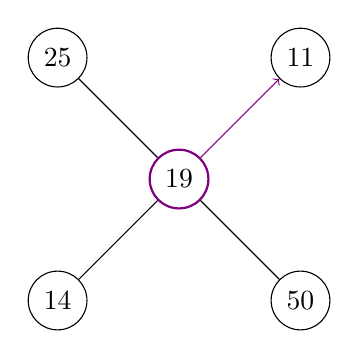
\begin{tikzpicture}[every node/.style={fill=white}, n/.style={circle, draw}]
        \node[n, thick, draw=violet] (s) at (0, 0) {19};
        \node[n] (n1) [above right=of s] {11};
        \node[n] (n2) [above left=of s] {25};
        \node[n] (n3) [below left=of s] {14};
        \node[n] (n4) [below right=of s] {50};

        \draw[->, violet] (s) edge (n1);
        \draw (s) edge (n2);
        \draw (s) edge (n3);
        \draw (s) edge (n4);
    \end{tikzpicture}

    \vspace{\baselineskip}

    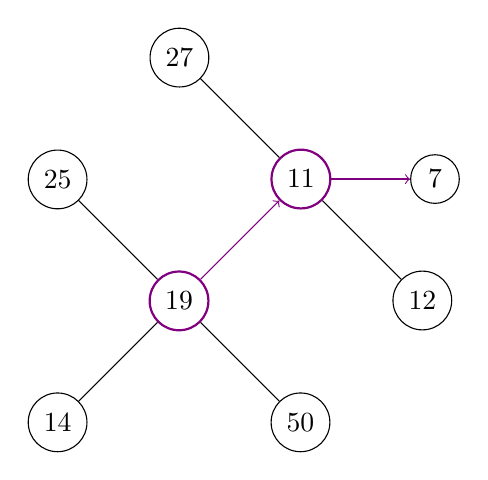
\begin{tikzpicture}[every node/.style={fill=white}, n/.style={circle, draw}]
        \node[n, thick, draw=violet] (s) at (0, 0) {19};
        \node[n, thick, draw=violet] (n1) [above right=of s] {11};
        \node[n] (n2) [above left=of s] {25};
        \node[n] (n3) [below left=of s] {14};
        \node[n] (n4) [below right=of s] {50};
        \node[n] (n5) [above left=of n1] {27};
        \node[n] (n6) [right=of n1] {7};
        \node[n] (n7) [below right=of n1] {12};

        \draw[->, violet] (s) edge (n1);
        \draw (s) edge (n2);
        \draw (s) edge (n3);
        \draw (s) edge (n4);
        \draw (n1) edge (n5);
        \draw[->, violet] (n1) edge (n6);
        \draw (n1) edge (n7);
    \end{tikzpicture}

    \vspace{\baselineskip}

    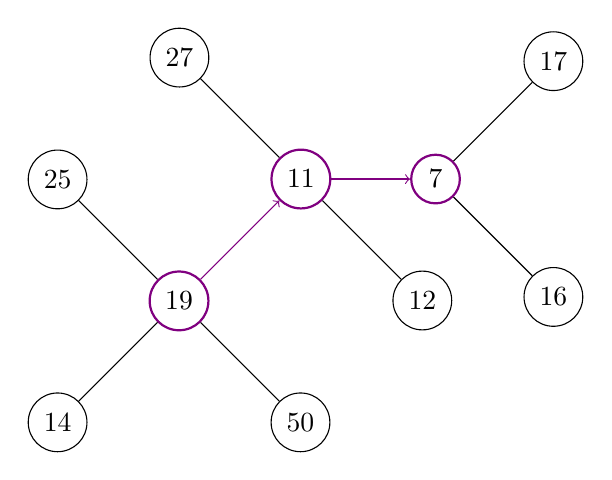
\begin{tikzpicture}[every node/.style={fill=white}, n/.style={circle, draw}]
        \node[n, thick, draw=violet] (s) at (0, 0) {19};
        \node[n, thick, draw=violet] (n1) [above right=of s] {11};
        \node[n] (n2) [above left=of s] {25};
        \node[n] (n3) [below left=of s] {14};
        \node[n] (n4) [below right=of s] {50};
        \node[n] (n5) [above left=of n1] {27};
        \node[n, thick, draw=violet] (n6) [right=of n1] {7};
        \node[n] (n7) [below right=of n1] {12};
        \node[n] (n8) [above right=of n6] {17};
        \node[n] (n9) [below right=of n6] {16};

        \draw[->, violet] (s) edge (n1);
        \draw (s) edge (n2);
        \draw (s) edge (n3);
        \draw (s) edge (n4);
        \draw (n1) edge (n5);
        \draw[->, violet] (n1) edge (n6);
        \draw (n1) edge (n7);
        \draw (n6) edge (n8);
        \draw (n6) edge (n9);
    \end{tikzpicture}
\end{example}

Ao final, o nó de valor $7$ é o mínimo local, então é a solução final.

A definição de vizinhança influencia no resultado.

É também importante tomar alguma decisões na hora de percorrer a vizinhança:

\begin{itemize}
    \item First fit - Ao percorrer os vizinhos, quando se encontra um que seja melhor que a solução atual, parte para ele.
    \item Best fit - Verifica \underline{todos} os vizinhos para escolher o melhor: guloso.
    \item Random - Busca aleatória. Mais variedade para encontrar mínimos locais diferentes.
\end{itemize}

Por exemplo, pode ser que depois do nó de valor $14$, exista uma solução melhor ainda.

\begin{example}
    \centering
    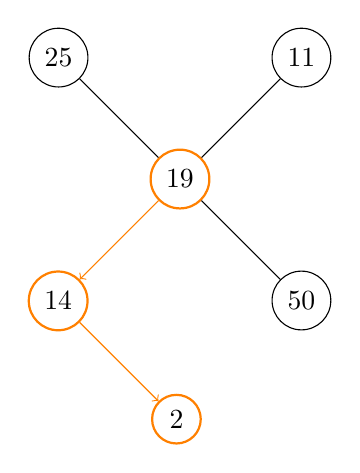
\begin{tikzpicture}[every node/.style={fill=white}, n/.style={circle, draw}]
        \node[n, thick, draw=orange] (s) at (0, 0) {19};
        \node[n] (n1) [above right=of s] {11};
        \node[n] (n2) [above left=of s] {25};
        \node[n, thick, draw=orange] (n3) [below left=of s] {14};
        \node[n] (n4) [below right=of s] {50};
        \node[n, thick, draw=orange] (n5) [below right=of n3] {2};

        \draw (s) edge (n1);
        \draw (s) edge (n2);
        \draw[->, orange] (s) edge (n3);
        \draw (s) edge (n4);
        \draw[->, orange] (n3) edge (n5);
    \end{tikzpicture}
\end{example}

First fit normalmente dá passos menores de melhoria, com mais passos. Já o best fit, dá menos passos maiores.

First fit pode ser mais eficiente, mas não necessariamente.

\newpage

\begin{algorithm}
\SetAlgoLined

$S \gets$ Solução inicial\;
\Enqto{Vizinhança da solução atual $S$ tiver uma solução $S'$ melhor}{
    $S \gets S'$\;
}
\Retorna S
\end{algorithm}

A solução inicial pode vir de uma heurística construtiva ou de soluções aleatórias.

Questões: como definir a vizinhança? Como percorrer a vizinhança?

\section{Problema do escalonamento}

\begin{itemize}
    \item \textbf{Entrada:} conjunto de tarefas $\{1, \dots , n\}$, cada tarefa $i$ tem tempo de processamento $t_i$ e $m$ máquinas idênticas.
    \item \textbf{Soluções viáveis:} partição das tarefas em $m$ conjuntos $\left\{ M_1, M_2, \dots , M_m\right\}$.
    \item \textbf{Função objetivo:} $\max\bar{j=1\dots m}\sum_{i \in M_j}t_i$ (makespan).
    \item \textbf{Objetivo:} econtrar solução de custo mínimo.
\end{itemize}

Vizinhança de um escalonamento $\mathcal{M}$: escalonamentos que diferem de $\mathcal{M}$ pela posição de um item.

Seja $l(j) = \sum_{i \in M_j} t_i$ a carga da máquina $j$.

\begin{algorithm}
\SetAlgoLined
\SetKwFunction{EscalonaUm}{EscalonaBuscaLocal}

\Fn{\EscalonaUm{n, t, m}}{
    $\mathcal{M} \gets $ um escalonamento inicial\;
    \tcc{$l(j')$ é o makespan atual}
    \Enqto{houver um item $i'$ na máquina mais carregada $j'$ e uma máquina $j$ tal que $l(j) + t_{i'} < l(j')$}{
        $M_{j'} \gets M_{j'} \setminus \left\{ i'\right\}$\;
        $M_j \gets M_j \cup \left\{ i'\right\}$\;
    }
    \Retorna $\max_{j=1, \dots , m}\sum_{i \in M_j}t_i$
}
\end{algorithm}

\newpage

\begin{example}

    \begin{center}
        $m=2$
    \end{center}

    \begin{multicols}{2}

        \tikzset{tempo/.style 2 args={rectangle split, rectangle split horizontal, draw=#2, rectangle split parts=#1, fill=#2!20}}

        \begin{center}
            \begin{tikzpicture}
                \node[tempo={1}{red}, label=below:$t_1$] (t1) at (0, 0) {};
                \node[tempo={1}{green}, label=below:$t_2$] (t2) [right=of t1] {};
                \node[tempo={2}{blue}, label=below:$t_3$] (t3) [right=of t2] {};
            \end{tikzpicture}
        \end{center}

        \begin{tabular}{l|l}
            $M_1$ & \tikzmark{4m11} \\
            $M_2$ & \tikzmark{4m21} \\
        \end{tabular}

        \begin{tikzpicture}[remember picture, tempo/.append style={anchor=west, overlay}, node distance=1pt]
            \node[tempo={1}{red}] (t1) at (pic cs:4m11) {};
            \node[tempo={1}{green}] (t2) [right=of t1] {};
            \node[tempo={2}{blue}] (t3) [right=of t2] {};
        \end{tikzpicture}

        \begin{center}
            \textit{makespan} = $4$
        \end{center}

        \begin{tabular}{l|l}
            $M_1$ & \tikzmark{5m11} \\
            $M_2$ & \tikzmark{5m21} \\
        \end{tabular}

        \begin{tikzpicture}[remember picture, tempo/.append style={anchor=west, overlay}, node distance=1pt]
            \node[tempo={1}{red}] (t1) at (pic cs:5m11) {};
            \node[tempo={1}{green}] (t2) [right=of t1] {};
            \node[tempo={2}{blue}] (t3) at (pic cs:5m21) {};
        \end{tikzpicture}

        \begin{center}
            \textit{makespan} = $2$
        \end{center}

        \columnbreak

        \begin{center}
            \begin{tikzpicture}
                \node[tempo={1}{red}, label=below:$t_1$] (t1) at (0, 0) {};
                \node[tempo={1}{green}, label=below:$t_2$] (t2) [right=of t1] {};
                \node[tempo={2}{blue}, label=below:$t_3$] (t3) [right=of t2] {};
            \end{tikzpicture}
        \end{center}

        \begin{tabular}{l|l}
            $M_1$ & \tikzmark{4m12} \\
            $M_2$ & \tikzmark{4m22} \\
        \end{tabular}

        \begin{tikzpicture}[remember picture, tempo/.append style={anchor=west, overlay}, node distance=1pt]
            \node[tempo={1}{red}] (t1) at (pic cs:4m12) {};
            \node[tempo={1}{green}] (t2) at (pic cs:4m22) {};
            \node[tempo={2}{blue}] (t3) [right=of t1] {};
        \end{tikzpicture}

        \begin{center}
            \textit{makespan} = $3$
        \end{center}

        \begin{tabular}{l|l}
            $M_1$ & \tikzmark{5m12} \\
            $M_2$ & \tikzmark{5m22} \\
        \end{tabular}

        \begin{tikzpicture}[remember picture, tempo/.append style={anchor=west, overlay}, node distance=1pt]
            \node[tempo={1}{green}] (t2) at (pic cs:5m22) {};
            \node[tempo={1}{red}] (t1) [right=of t2] {};
            \node[tempo={2}{blue}] (t3) at (pic cs:5m12) {};
        \end{tikzpicture}

        \begin{center}
            \textit{makespan} = $2$
        \end{center}
    \end{multicols}
\end{example}

No seguinte exemplo, não há nenhum movimento possível que melhore o resultado.

\begin{example}
    \begin{center}
        $m=2$
    \end{center}

    \tikzset{tempo/.style 2 args={rectangle split, rectangle split horizontal, draw=#2, rectangle split parts=#1, fill=#2!20}}

    \begin{center}
        \begin{tikzpicture}[node distance=.25cm]
            \node[tempo={3}{orange}] (t1) at (0, 0) {};
            \node[tempo={2}{blue}] (t2) [right=of t1] {};
            \node[tempo={2}{red}] (t3) [right=of t2] {};
            \node[tempo={3}{green}] (t4) [right=of t3] {};
            \node[tempo={2}{violet}] (t5) [right=of t4] {};
        \end{tikzpicture}
    \end{center}

    \begin{tabular}{l|l}
        $M_1$ & \tikzmark{6m11} \\
        $M_2$ & \tikzmark{6m21} \\
    \end{tabular}

    \begin{tikzpicture}[remember picture, , tempo/.append style={anchor=west, overlay}, node distance=1pt]
        \node[tempo={3}{orange}] (t1) at (pic cs:6m11) {};
        \node[tempo={3}{green}] (t2) at (pic cs:6m21) {};
        \node[tempo={2}{blue}] (t3) [right=of t1] {};
        \node[tempo={2}{red}] (t4) [right=of t2] {};
        \node[tempo={2}{violet}] (t5) [right=of t3] {};
    \end{tikzpicture}

    \textit{makespan} = $7$
\end{example}

Trocando o conceito de vizinhança para lidar com dois itens de diferença, nós conseguimos encontrar uma solução melhor.

\begin{example}
    \tikzset{tempo/.style 2 args={rectangle split, rectangle split horizontal, draw=#2, rectangle split parts=#1, fill=#2!20}}

    \begin{tabular}{l|l}
        $M_1$ & \tikzmark{7m11} \\
        $M_2$ & \tikzmark{7m21} \\
    \end{tabular}

    \begin{tikzpicture}[remember picture, , tempo/.append style={anchor=west, overlay}, node distance=1pt]
        \node[tempo={2}{red}] (t4) at (pic cs:7m11) {};
        \node[tempo={3}{green}] (t2) at (pic cs:7m21) {};
        \node[tempo={3}{orange}] (t1) [right=of t2] {};
        \node[tempo={2}{blue}] (t3) [right=of t4] {};
        \node[tempo={2}{violet}] (t5) [right=of t3] {};
    \end{tikzpicture}

    \textit{makespan} = $6$
\end{example}

\begin{algorithm}
\SetAlgoLined
\SetKwFunction{EscalonaDois}{EscalonaBuscaLocal2}

\Fn{\EscalonaDois{n, t, m}}{
    $\mathcal{M} \gets$ um escalonamento inicial\;
    \Enqto{houver $i'$ na máquina mais carregada $j'$ e $i$ numa máquina $j$ tal que $l(j) - t_i + t_{i'} < l(j')$ e $l(j') - t_{i'}+t_i<l(j')$}{
        $M_{j'}\gets M_{j'} \setminus \{i'\} \cup \left\{ i\right\}$\;
        $M_j \gets \left\{ i\right\} \cup \left\{ i'\right\}$\;
    }
    \Retorna $\max_{j=1,\dots ,m}\sum_{i \in M_j}t_i$
}
\end{algorithm}

Normalmente as diferentes vizinhanças são combinadas. Iniciando com as vizinhanças mais simples e, quando não dá pra melhorar nada com elas, usa as vizinhanças mais complexas.

\section{Problema do Corte Máximo}

\begin{itemize}
    \item \textbf{Entrada:} um grafo $G = (V, E)$.
    \item \textbf{Soluções viáveis:} um corte de $G$, i.e., um conjunto $S$ tal que $\emptyset\neq S \subset V$.
    \item \textbf{Função objetivo:} número de arestas que sai de $S$, i.e., $|\delta(S)|$.
    \item \textbf{Objetivo:} encontrar solução de custo máximo.
\end{itemize}

Vizinhança de um corte $S$: cortes que tem apenas um vértice a mais ou a menos que $S$.

$c(v) = $ número de arestas incidentes a $v$ que atravessam o corte.

$d(v) = $ número de arestas incidentes a $v$ que não atravessam o corte.

\begin{algorithm}
\SetAlgoLined
\SetKwFunction{CorteUm}{CorteMaximoBuscaLocal}

\Fn{\CorteUm{$G=(V, E)$}}{
    $S \gets $ um corte inicial\;
    $\bar{S} \gets V \setminus S$\;

    \Enqto{houver vértice v tal que $c(v) < d(v)$}{
        \eSe{$v \in S$}{
            $S \gets S \setminus \left\{ v\right\}$\;
            $\bar{S} \gets \bar{S} \cup \left\{ v\right\}$\;
        }{
            $\bar{S} \gets \bar{S} \setminus \left\{ v\right\}$\;
            $S \gets S \cup \left\{ v\right\}$\;
        }
    }
    \Retorna S
}
\end{algorithm}

\begin{example}
    \centering
    \begin{tikzpicture}[every node/.style={fill=white}, n/.style={circle, draw}, scale=.8]
        \node[n] (a) at (0.5, 2) {a};
        \node[n] (b) at (3, 0) {b};
        \node[n] (c) at (2, -3) {c};
        \node[n] (d) at (-1, -3) {d};
        \node[n] (e) at (-2, 0) {e};

        \draw (a) edge (b);
        \draw (a) edge (c);
        \draw (b) edge (c);
        \draw (c) edge (d);
        \draw (d) edge (e);
        \draw (e) edge (a);
    \end{tikzpicture}

    \vspace{\baselineskip}

    \begin{tikzpicture}[every node/.style={fill=white}, n/.style={circle, draw}]
        \node[n] (a) at (0, 0) {a};
        \node[n] (c) [below=of a] {c};
        \node[n] (e) [below=of c] {e};
        \node[n] (b) at (4, 0) {b};
        \node[n] (d) [below=of b] {d};

        \node[fill=none, draw, ellipse, fit=(a)(c)(e), label=above:$S$] {};
        \node[fill=none, draw, ellipse, fit=(b)(d), label=above:$\bar{S}$] {};

        \draw[thick, red] (a) edge (b);
        \draw (a) edge (c);
        \draw[thick, red] (b) edge (c);
        \draw[thick, red] (c) edge (d);
        \draw[thick, red] (d) edge (e);
        \draw (e) to[out=120, in=-120] (a);
    \end{tikzpicture}

    $c(a) = 1 < 2 = d(a)$

    \vspace{\baselineskip}
    
    \begin{tikzpicture}[every node/.style={fill=white}, n/.style={circle, draw}]
        \node[n] (a) at (4, 0) {a};
        \node[n] (c) at (0, 0) {c};
        \node[n] (e) [below=of c] {e};
        \node[n] (b) [below=of a] {b};
        \node[n] (d) [below=of b] {d};

        \node[fill=none, draw, ellipse, fit=(c)(e), label=above:$S$] {};
        \node[fill=none, draw, ellipse, fit=(a)(b)(d), label=above:$\bar{S}$] {};

        \draw (a) edge (b);
        \draw[thick, red] (a) edge (c);
        \draw[thick, red] (b) edge (c);
        \draw[thick, red] (c) edge (d);
        \draw[thick, red] (d) edge (e);
        \draw[thick, red] (e) edge (a);
    \end{tikzpicture}
\end{example}

Nesse caso, a heurística de busca local melhorou o resultado obtido pelo algoritmo guloso.

\section{Problema da Localicação de Instalações}

Localização de Instalações \underline{sem Capacidades} $\to$ UFL

\begin{itemize}
    \item \textbf{Entrada:} conjunto de clientes $D$, conjunto de instalações $F$, distância $d: D \times F \mapsto \mathbb{R}^+$ e custo de abertura $f: F \mapsto \mathbb{R}^+$.
    \item \textbf{soluções viáveis:} um subconjunto $F'$, tal que $\emptyset \neq F' \subseteq F$.
    \item \textbf{Função objetivo:} custo de abertura mais custo de conexão, i.e., $\sum_{i \in F'} f(i) + \sum_{j \in D}d(j, a(j))$, com $a(j)$ instalação mais próxima de $j$ em $F'$.
    \item \textbf{Objetivo:} encontrar solução de custo mínimo.
\end{itemize}

 Vizinhança de um conjunto de instalações $F'$: conjuntos que tem apenas uma instalação a mais ou a menos que $F'$.

 $D(i) = $ conjunto de clientes mais próximos de $i$ que de qualquer instalação em $F'$. $\to i$ não está em $F'$, mas atrairia esses clientes se estivesse.

 $\Delta(i) = \sum_{j \in D_j}d(j, a(j)) - \sum_{j \in D_i} d(j, i)$. $\to$ Ganho de conexão.

 \begin{algorithm}
 \SetAlgoLined
 \SetKwFunction{UFLUm}{UFL-BuscaLocal}
 \Fn{\UFLUm{D, F, d, f}}{
     $F' \gets $ um conjunto inicial de instalações\;
     \Enqto{houver uma instalação $i'$ tal que $i'\in F'$ com $f(i') > \Delta(i')$ ou $i'\in F \setminus F'$ com $f(i') < \Delta(i')$}{
         \eSe{$i'\in F'$}{
             \tcc{$i'$ não se paga}
             $F' \gets F' \setminus \left\{ i'\right\}$\;
         }{
             \tcc{$i'$ deveria estar aberto}
             $F' \gets F' \cup \left\{ i'\right\}$\;
         }
     }
     \Retorna $F'$
 }
 \end{algorithm}

 \begin{example}
     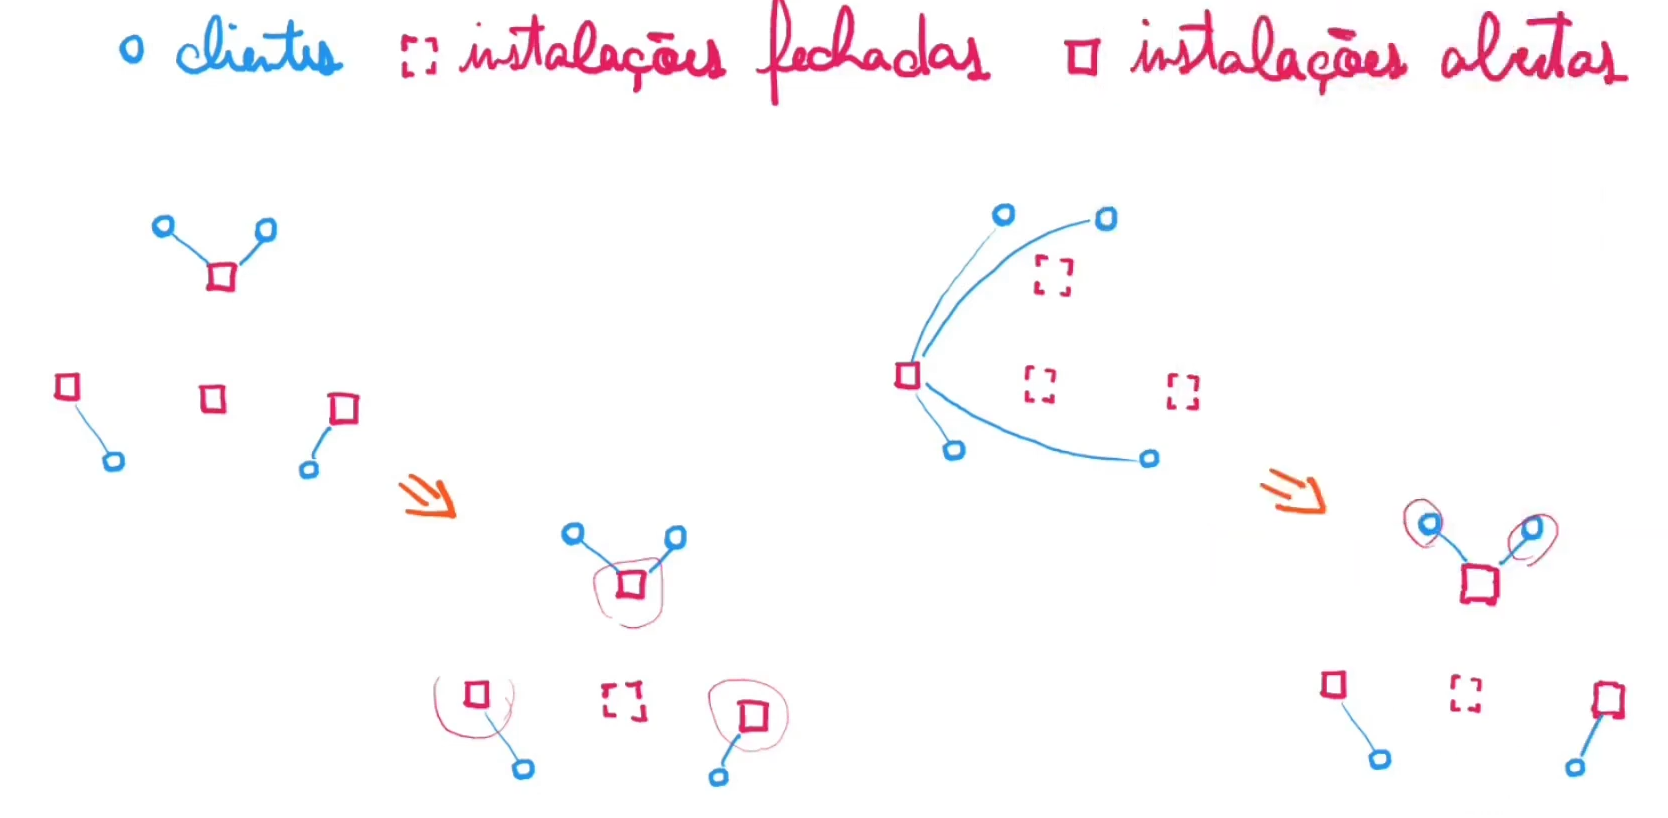
\includegraphics[width=.8\textwidth]{img/localizacao_instalacoes.png}
 \end{example}

 \section{Problema do caixeiro viajante}

 \begin{itemize}
     \item \textbf{Entrada:} $G = (V, E)$ e função $w$ de peso nas arestas.
     \item \textbf{Soluções viáveis:} circuitos hamiltonianos de $G$.
     \item \textbf{Função objetivo:} soma dos pesos das arestas do circuito.
     \item \textbf{Objetivo:} encontrar um circuito de menor custo.
 \end{itemize}

 Vizinhança 2-OPT de um circuito hamiltoniano $C$: conjunto dos circuitos hamiltonianos que são obtidos trocando 2 arestas de $C$.

 \begin{example}
    \centering
    \begin{multicols}{3}
        \begin{tikzpicture}[every node/.style={fill=white}, n/.style={circle, draw}]
            \node[n] (c) at (0, 0) {c};
            \node[n] (b) at (1, 1) {b};
            \node[n] (d) at (1, -1) {d};
            \node[n] (a) at (2, 1) {a};
            \node[n] (e) at (2, -1) {e};
            \node[n] (h) at (3, 1) {h};
            \node[n] (f) at (3, -1) {f};
            \node[n] (g) at (4, 0) {g};

            \draw (c) edge (b);
            \draw (b) edge (e);
            \draw (e) edge (f);
            \draw (f) edge (g);
            \draw (g) edge (h);
            \draw (h) edge (a);
            \draw (a) edge (d);
            \draw (d) edge (c);
        \end{tikzpicture}
        \columnbreak
        \vspace*{.8cm}
        {\Huge $\Rightarrow$}
        \columnbreak
        \begin{tikzpicture}[every node/.style={fill=white}, n/.style={circle, draw}]
            \node[n] (c) at (0, 0) {c};
            \node[n] (b) at (1, 1) {b};
            \node[n] (d) at (1, -1) {d};
            \node[n] (a) at (2, 1) {a};
            \node[n] (e) at (2, -1) {e};
            \node[n] (h) at (3, 1) {h};
            \node[n] (f) at (3, -1) {f};
            \node[n] (g) at (4, 0) {g};

            \draw (c) edge (b);
            \draw (b) edge (a);
            \draw (e) edge (f);
            \draw (f) edge (g);
            \draw (g) edge (h);
            \draw (h) edge (a);
            \draw (e) edge (d);
            \draw (d) edge (c);
        \end{tikzpicture}
    \end{multicols}
\end{example}

É importante garantir que a troca permita que a solução seja ainda viável. Por exemplo, a troca a seguir \underline{não} pode ser feita.

\begin{example}
    \centering
    \begin{multicols}{3}
        \begin{tikzpicture}[every node/.style={fill=white}, n/.style={circle, draw}]
            \node[n] (c) at (0, 0) {c};
            \node[n] (b) at (1, 1) {b};
            \node[n] (d) at (1, -1) {d};
            \node[n] (a) at (2, 1) {a};
            \node[n] (e) at (2, -1) {e};
            \node[n] (h) at (3, 1) {h};
            \node[n] (f) at (3, -1) {f};
            \node[n] (g) at (4, 0) {g};

            \draw (c) edge (b);
            \draw (b) edge (e);
            \draw (e) edge (f);
            \draw (f) edge (g);
            \draw (g) edge (h);
            \draw (h) edge (a);
            \draw (a) edge (d);
            \draw (d) edge (c);
        \end{tikzpicture}
        \columnbreak
        \vspace*{.8cm}
        {\Huge $\Rightarrow$}
        \columnbreak
        \begin{tikzpicture}[every node/.style={fill=white}, n/.style={circle, draw}]
            \node[n] (c) at (0, 0) {c};
            \node[n] (b) at (1, 1) {b};
            \node[n] (d) at (1, -1) {d};
            \node[n] (a) at (2, 1) {a};
            \node[n] (e) at (2, -1) {e};
            \node[n] (h) at (3, 1) {h};
            \node[n] (f) at (3, -1) {f};
            \node[n] (g) at (4, 0) {g};

            \draw (c) edge (b);
            \draw (e) edge (a);
            \draw (e) edge (f);
            \draw (f) edge (g);
            \draw (g) edge (h);
            \draw (h) edge (a);
            \draw (b) edge (d);
            \draw (d) edge (c);
        \end{tikzpicture}
    \end{multicols}
\end{example}

\begin{algorithm}
\SetAlgoLined
\SetKwFunction{TSPCinco}{TSP-2-OPT}
\Fn{\TSPCinco{$G=(V, E), w$}}{
    $C \gets$ um circuito hamiltoniano inicial\;
    \Enqto{houver um par de arestas $(u, v)$ e $(x, z)$ em $C$ tal que $w(u, x) + w(x, z) < w(u, v) + w(x, z)$}{
        $C \gets C \setminus \left\{ (u, v), (x, z)\right\} \cup \left\{ (u, x), (v, z)\right\}$\;
    }
    \Retorna C
}
\end{algorithm}

É possível utilizar uma vizinhança 3-OPT.

\begin{example}
    \centering
    \begin{tikzpicture}[every node/.style={fill=white}, n/.style={circle, draw}]
        \node[n] (a) at (0, 0) {a};
        \node[n] (b) at (-2, -1) {b};
        \node[n] (c) at (-4, -2) {c};
        \node[n] (d) at (-2, -3) {d};
        \node[n] (e) at (0, -4) {e};
        \node[n] (f) at (2, -3) {f};
        \node[n] (g) at (4, -2) {g};
        \node[n] (h) at (2, -1) {h};

        \draw (a) edge (b);
        \draw (b) edge (e);
        \draw (e) edge (d);
        \draw (d) edge (c);
        \draw (c) edge (h);
        \draw (h) edge (g);
        \draw (g) edge (f);
        \draw (f) edge (a);
    \end{tikzpicture}

    \vspace{\baselineskip}
    
    {\Huge $\Downarrow$}
    
    \vspace{\baselineskip}
    
    \begin{tikzpicture}[every node/.style={fill=white}, n/.style={circle, draw}]
        \node[n] (a) at (0, 0) {a};
        \node[n] (b) at (-2, -1) {b};
        \node[n] (c) at (-4, -2) {c};
        \node[n] (d) at (-2, -3) {d};
        \node[n] (e) at (0, -4) {e};
        \node[n] (f) at (2, -3) {f};
        \node[n] (g) at (4, -2) {g};
        \node[n] (h) at (2, -1) {h};

        \draw (a) edge (b);
        \draw (b) edge (c);
        \draw (c) edge (d);
        \draw (d) edge (e);
        \draw (e) edge (f);
        \draw (f) edge (g);
        \draw (g) edge (h);
        \draw (h) edge (a);
    \end{tikzpicture}
\end{example}

Na realidade é possível usar uma vizinhança k-OPT mais geral. Uma \textbf{categoria de vizinhanças}.

\section{Metaheurísticas de busca}
\label{sec:metaheuristicas}

Extensões da busca local. Como fugir do mínimo local?

\begin{itemize}
    \item Repeated local search
    \item Simulated annealing
    \item Tabu search
    \item Variable neighbourhood search
    \item GRASP
\end{itemize}

\subsection{Repeated local search}

Realizar diversas buscas locais com instâncias e buscas aleatórias. Joga diferentes pontos iniciais de busca, para que alguma delas encontre uma solução razoável.

\begin{center}
    \def\svgwidth{.75\linewidth}
    \import{img/}{repeated_local_search.pdf_tex}
\end{center}

\newpage

\subsection{Simulated annealing (Cozimento simulado)}

Ideia de temperatura. Enquanto a temperatura do sistema está alta, a busca tem grande chance de fazer escolhas que piorem a solução.

O algoritmo busca o espaço ao redor da solução inicial de forma mais aleatória (podendo ir para soluções piores), mas conforme o tempo passa (temperatura abaixa), converge para um mínimo local.

\begin{center}
    \def\svgwidth{.75\linewidth}
    \import{img/}{simulated_annealing.pdf_tex}
\end{center}

\subsection{Tabu seach}

No início faz uma busca local até um mínimo local. Chegando no mínimo, ele passa a aceitar vizinhos que piorem para escapar do mínimo local. Espera encontrar em algum ponto um mínimo local melhor que o anterior.

\begin{center}
    \def\svgwidth{.75\linewidth}
    \import{img/}{tabu_search.pdf_tex}
\end{center}

Existe uma questão que, enquanto ``sobe o morro'', sempre há pelo menos uma solução melhor (a que você veio antes). Para isso, tem que ter uma lista tabu indicando que soluções já percorreu e proibir essses movimentos.

\subsection{Variable neighbourhood search}

Usa uma vizinhança mais simples. Quando chega em um mínimo local, usa uma vizinhança mais complexa e depois volta para a vizinhança mais simples. Pode usar diversos níveis de complexidade de vizinhanças.

\subsection{GRASP - Greed Randomized Adaptive Search Procedure}

Combina estratégia gulosa com aleatoriedade e busca local. Aleatoriza os algoritmos gulosos para que cada vez que executa, ele percorra um caminho diferente trazendo diversidade de soluções. Em cada passo, tem também um processo de busca local para melhorar o resultado obtido pelo algoritmo guloso.

\chapter{Programação Linear Inteira}

Está dentro dos métodos exatos. Abre mão do tempo polinomial para o pior caso, mas obtém sempre a solução ótima. Exemplos:

\begin{itemize}
    \item Programação dinâmica
    \item \textit{Branch and bound}
    \item Programação linear (inteira)
    \item Programação por restrições
\end{itemize}

\section{Definição}

Modelo matemático que descreve problemas de otimização combinatória.

\begin{itemize}
    \item Um conjunto de variáveis inteiras
    \item Um conjunto de restrições (inequações lineares)
    \item Uma função objetivo (expressão \underline{linear})
\end{itemize}

Solução viável: atribuição para as variáveis. Desde que satisfazam as restrições.

\begin{example}
    Existem também problemas mistos: com variáveis inteiras e contínuas.
\end{example}

\subsection{Forma genérica de um PLI}

\begin{example}
    $n$ variáveis
    
    $m$ restrições
    
    minimizar $\sum_{j=1}^n c_jx_j$
    
    sujeito a $\sum_{j=1}^n a_{ij}x_j\geq b_i, \forall i \in \left\{ 1,\dots , m\right\}$
    
    $x_j \in \mathbb{Z}^+, \forall j \in \left\{ 1, \dots ,n\right\}$
\end{example}

$a_{ij}, b_i$ e $c_j$ são constantes e $x_j$ são as variáveis.

Função objetivo: $\sum_{j=1}^n c_jx_j$.

Se multiplicar a função objetivo por $-1$, o problema de minimização se torna de maximização. Igualmente, para as restrições, pode multiplicar por $-1$ para obter uma inequação ``menor que'' ($\leq$). Para garantir a igualdade, usamos duas inequações:

\[
    \sum_{j=1}^n a_{ij}x_j = b_i \iff
    \begin{cases}
        \sum_{j=1}^n a_{ij}x_j \geq b_i \\
        \sum_{j=1}^n a_{ij}x_j \leq b_i
    \end{cases}
\]

É comum usar \underline{variáveis binárias}.

\subsection{Programa linear}

Pode-se fazer uma ``relaxação da integridade'' para obter um Programa Linear (PL), em que as variáveis deixam de ser inteiras e podem ser reais.

Um programa linear inteiro sempre pode ser ``relaxado'' para um PL. Com isso, podemos garantir que o PL é um \textbf{limitante} do PLI original.

\underline{Toda solução do PLI é uma solução do PL.}

PL podem ser resolvidos em tempo polinomial. (PLI não garante isso)

Resolvedores de PLI normalmente combinam \textit{branch and bound} com Pl. Para encontrar melhores limitantes inferiores e realizar mais podas na árvore de busca.

\section{Problema da Mochila Binária}

\begin{itemize}
    \item Variáveis: $x_i \quad i = 1,\dots ,n$ binária, indicando se o item $i$ está na mochila.
    \item Função objetivo: $\max\sum_{i=1}^n v_ix_i$. Maximizar o valor da mochila
    \item Restrição: $\sum_{i=1}^n w_ix_i \leq W$. O peso máximo da mochila deve ser respeitado.
\end{itemize}

Qual o problema obtido ao se relaxar a restrição de integralidade dos $x_i$? $\to$ Mochila Fracionária

\section{Problema do Escalonamento}

\begin{itemize}
    \item Variáveis: $x_{ij} \quad i = 1,\dots,n \quad j=1,\dots,m$ binária indicando se a tarefa $i$ está na máquina $j$.
    \item $L_{\max}$. Variável que representa o makespan.
    \item Função objetivo: $\min L_{\max}$. Minimizar o \textit{makespan}.
    \item Restrições:
    \begin{itemize}
        \item $\sum_{j=1}^mx_{ij}=1$. Cada tarefa está alocada em uma única máquina.
        \item $\sum_{i=1}^nt_ix_{ij}\leq L_{\max} \quad j=1,\dots,m$. O \textit{makespan} tem que ser $\geq$ à carga de qualquer máquina.
    \end{itemize}
    \item Domínio das variáveis:
    \begin{itemize}
        \item $x_{ij} \in \{0,1\} \quad i=1,\dots,n \quad j=1,\dots,m$
        \item $L_{\max} \in \mathbb{R}$
    \end{itemize}
\end{itemize}

É um problema de Programação Linear misto, porque tem variáveis inteiras ($x_{ij}$) e contínuas ($L_{\max}$) junto.

\section{Problema da Colocação de Grafos}

\begin{itemize}
    \item Variáveis:
    \begin{itemize}
        \item $x_{uk} \quad u \in V \quad k = 1,\dots,\Delta(G)+1$. Indica se o vértice $u$ tem cor $k$. $\Delta(G)$ é o grau máximo no grafo.
        \item $y_k \quad k=1,\dots,\Delta(G)+1$. Indica se a cor $k$ é usada.
    \end{itemize}
    \item Função objetivo: $\min\sum_{k=1}^{\Delta(G)+1}y_k$. Minimizar o número de cores usadas.
    \item Restrições:
    \begin{itemize}
        \item $\sum_{k=1}^{\Delta(G)+1} x_{uk} = 1 \quad \forall u\in V$. Cada vértice tem apenas uma cor.
        \item $x_{uk}+x_{vk} \leq 1 \quad \forall (u,v) \in E \quad k=1,\dots,\Delta(G)+1$. Vértices adjacentes tem cores diferentes.
        \item $x_{uk} \leq y_k \quad \forall u \in V \quad k=1,\dots,\Delta(G)+1$. Um vértice só pode usar uma cor que esteja disponível (cujo $y_k=1$).
    \end{itemize}
    \item Domínio das variáveis:
    \begin{itemize}
        \item $x_{uk} \in \{0, 1\} \quad u \in V \quad k = 1,\dots,\Delta(G)+1$
        \item $y_k \in \{0,1\} \quad k = 1,\dots,\Delta(G)+1$
    \end{itemize}
\end{itemize}

O número máximo de cores é $\Delta(G) + 1$ porque o pior caso é quando o nó com maior grau tem todos os vizinhos com cores diferentes, então ele precisa ser colorido com uma cor nova.

\section{Problema da Localização de Instalações sem Capacidades}

\begin{itemize}
    \item Variáveis:
    \begin{itemize}
        \item $y_i \quad i \in F$. Indica se a instalação $i$ foi aberta.
        \item $x_{ij} \quad i \in F \quad j \in D$. Indica se cliente $j$ se conecta à instalação $i$.
    \end{itemize}
    \item Função objetivo: $\min\sum_{i \in F} f_iy_i + \sum_{j\in D}\sum_{i \in F} d_{ji}x_{ij}$. Minimizar o custo de abertura mais custo de conexão.
    \item Restrições:
    \begin{itemize}
        \item $\sum_{i \in F}x_{ij}=1 \forall j \in D$. Cada cliente se conecta a apenas uma instalação.
        \item $x_{ij}\leq y_i \quad \forall i \in F \quad \forall j \in D$. Cliente só pode se conectar a uma instalação aberta.
    \end{itemize}
    \item Domínio das variáveis:
    \begin{itemize}
        \item $x_{ij} \{0,1\} \quad \forall i \in F \quad \forall j \in D$
        \item $y_i \in \{0,1\} i \in F$
    \end{itemize}
\end{itemize}

\section{Problema da Cobertura por Conjuntos}

\begin{itemize}
    \item \textbf{Entrada:} conjunto de elementos $U = \{e_1,e_2,\dots,e_n\}$, uma coleção de subconjuntos $S_1,S_2,\dots,S_m$, cada subconjunto $S_j \subseteq U$ com peso $w_j$.
    \item \textbf{Soluções viáveis:} uma coleção de subconjuntos que cobre $U$, i.e., encontrar $I \subseteq \{1,2,...,m\}$ tal que $\bigcup_{j \in I} S_j = U$.
    \item \textbf{Função objetivo:} custo total dos subconjuntos em $I$, i.e., $\sum_{j \in I}w_j$.
    \item \textbf{Objetivo:} encontrar coleção de custo mínimo.
\end{itemize}

\subsection{Formulação em PLI}

\begin{itemize}
    \item Variáveis: $x_j \quad j=1,\dots,m$. Indica se o conjunto $j$ foi escolhido.
    \item Função objetivo: $\min\sum_{j=1}^mw_jx_j$. Minimizar o custo dos subconjuntos escolhidos.
    \item Restrição: $\sum_{j:e_i \in S_j}x_j\geq 1\quad i=1,\dots,n$. Todo elemento deve ser coberto por ao menos um subconjunto.
    \item Domínio das variáveis: $x_j \in \{0,1\} \quad j=1,...,m$
\end{itemize}

\section{Resolvedores de PLI}

Ferramenta para fazer a modelagem de PLI: OR-tools. Gratuito.

Resolvedores mais famosos: Gurobi, CPLEX. São resolvedores proprietários.

\subsection{OR-Tools}

Usar o \lstinline{pywraplp} do \lstinline{ortools.linear_solver}. Usar um resolvedor \lstinline{pywraplp.Solver}.

O que tem que fazer é criar as variáveis em uma lista.

\begin{lstlisting}
x = list()
for j in range(0, num_sets):
    # Variaveis inteiras entre 0 e 1 = binarias
    # Toda variavel tem um nome x[j]
    x.append(solver.IntVar(0.0, 1.0, 'x[{}]'.format(j)))
\end{lstlisting}

Depois, criamos as restrições (\textit{constraints}) para cada elemento $e_i \in U$.

\begin{lstlisting}
constraintType1 = list()
for i in range(0, num_elements):
    # Um constraint tem dois limitantes (inferior e superior)
    constraintType1.append(solver.Constraint(1, solver.infinity()))
\end{lstlisting}

Na parte direita da inequação ($\sum_{j:e_i \in S_j}$), nós levamos em consideração todos os conjuntos que possuem o elemento $e_i$. Então temos que passar por todos os conjuntos e seus elementos para indicar a restrição, aplicar aquele \textit{constraint} para aquele conjunto em específico (colocar o coeficiente como $1$).

\begin{lstlisting}
for s in set_list:
    for i in s.elements:
        constraintType1[i].Setcoefficient(x[s.index], 1)
\end{lstlisting}

Também temos que definir a função objetivo.

\begin{lstlisting}
objective = solver.Objective()
objective.SetMinimization() # A funcao eh de minimizacao
for j in range(0, num_sets):
    objective.SetCoefficient(x[j], set_list[j].cost)
\end{lstlisting}

Depois de modelado, podemos apenas resolver usando \lstinline{solver.Solve()}

\section{Problema do corte máximo}

\begin{itemize}
    \item Variáveis:
    \begin{itemize}
        \item $x_u \quad \forall u \in V$. Indica se o vértice $u$ esta no corte $S$.
        \item $y_e \quad \forall e \in E$. Indica se a aresta atravessa o corte $S$.
    \end{itemize}
    \item Função objetivo: $\max\sum_{e \in E} y_e$. Maximizar o número de arestas no corte.
    \item Restrições:
    \begin{itemize}
        \item $y_e \leq x_u - x_v + M \times a_e \quad \forall e=(u,v)\in E$. A aresta só atravessa o corte se os extremos estão em grupos distintos (direção $u \to v$).
        \item $y_e \leq x_v - x_u + M \times (1-a_e) \quad \forall e=(u, v) \in E$. Direção $v \to u$.
    \end{itemize}
    \item Domínio das variáveis:
    \begin{itemize}
        \item $x_u \in \{0,1\} \quad \forall u \in V$
        \item $y_e \in \{0,1\} \quad \forall e \in E$
        \item $a_e \in \{0,1\} \quad \forall e \in E$
    \end{itemize}
\end{itemize}

Usa o $M$, \underline{um número grande}, e uma variável auxiliar $a_e$ binária associada a cada aresta. Isso seleciona apenas uma das restrições a funcionar em cada tempo (tipo o módulo, mas módulo \textbf{não} é função linear). São duas restrições complementares. Por ser uma variável, o resolvedor vai escolher os melhores valores para $a_e$ para garantir o resultado.

\section{Problema de Steiner}

\begin{itemize}
    \item \textbf{Entrada:} $G = (V, E)$, com $V = R \cup S$, sendo $R$ terminais e $S$ vértices de Steiner, e função $w$ de peso nas arestas.
    \item \textbf{Soluções viávies:} árvores que conectam todos os vértices em $R$.
    \item \textbf{Função objetivo:} soma dos pesos das arestas na árvore.
    \item \textbf{Objetivo:} encontrar uma árvore de peso mínimo.
\end{itemize}

\subsection{Formulação em PLI}

\begin{itemize}
    \item Variáveis: $x_e \quad \forall e \in E$. Indica se a aresta $e$ está na árvore.
    \item Função objetivo: $\min\sum_{e \in E}w_ex_e$. Minimizar o custo da árvore.
    \item Restrições: $\sum_{e \in \delta(S)} x_e\geq 1\quad \forall S:S\cap R \neq\emptyset, S\cap R \subset R$ Qualquer corte $S$ que separa os terminais deve ter aresta atravessando.
    \item Domínio das variáveis: $x_e \in \{0,1\} \quad \forall e \in E$.
\end{itemize}
\chapter{Programação Linear - Continuação}

Garante a solução ótima, mas sem garantir o tempo polinomial.

\section{Programação linear}

Diferente do PLI, aqui as variáveis podem ser \textbf{reais}, não necessariamente inteiras.

As variáveis são sempre positivas. Se precisar de variáveis que possam ser negativas, usa-se duas variáveis na verdade, sempre em dupla ($x_i^+ - x_i^-$). A combinação das duas variáveis podem gerar os valores positivos ou negativos necessários.

\subsection{Exepmlo de PL para produção}

Dois tipos de produto. Cada produto do tipo 1 dá 1 de lucro, e cada produto do tipo 2 dá 2 de lucro.

Maximizar: $x_1 + 2x_2$

Mas existem insumos (restrições).

\begin{itemize}
    \item $x_1 \leq 7 \to \alpha$
    \item $x_2 \leq 5 \to \beta$
    \item $2x_1 + x_2 \leq 16 \to \gamma$
    \item $-x_1 + x_2 \leq 3 \to \delta$
\end{itemize}

A produção também não pode ser negativa.

\begin{itemize}
    \item $x_1 \geq 0$
    \item $x_2 \geq 0$
\end{itemize}

É possível visualizar as restições no plano.

\begin{example}
    \begin{center}
        \def\svgwidth{.75\linewidth}
        \import{img/}{grafico_pl.pdf_tex}
    \end{center}
\end{example}

A função objetivo é representada por um vetor (o que importa é o comprimento, direção e sentido). Esse vetor é ortogonal a uma reta em que $x_1 + 2x_2$ é constante. Ao longo dessa  reta, o valor da função objetivo não muda.

\section{Intuição geométrica do Simplex}

A ideia é migrar de um vértice para um vértice vizinho do poliedro (a área dentro das restrições) sempre melhorando a função objetivo. $\to$ \textbf{Busca local}

\begin{example}
    \begin{center}
        \def\svgwidth{.75\linewidth}
        \import{img/}{grafico_simplex.pdf_tex}
    \end{center}
\end{example}

Iniciando no ponto $(0, 0)$, vamos aumentando o valor de $x_1$ e, em seguida, o valor de $x_2$, já que o vetor da função objetivo indica que o valor aumenta conforme aumenta o $x_1$ e, mais ainda, o $x_2$.

Depois nós voltamos, porque, apesar de diminuir o valor de $x_1$, $x_2$ contribui mais para o valor da função objetivo. E chegamos então ao máximo local. Os únicos dois vizinhos são o ponto de onde veio $(7, 2)$ e o ponto seguinte $(2, 5)$. Mas os dois têm valores piores que o ponto atual.

\subsection{Convexidade}

Essa estratégia funciona pois o poliedro é convexo (qualquer segmento de reta ligando dois pontos do conjunto está dentro do conjunto).

Todo conjunto definido pelas restrições lineares (chamado de semi-espaço) é convexo. Porque o formato das restrições são sempre ``os pontos que estão acima (ou abaixo) desse plano''. E a intersecção de duas ou mais restrições também é convexa. Então \textbf{todo} poliedro resultante é convexo.

Como o poliedro é convexo, \textbf{todo ótimo local é ótimo global}. E isso também garante que \textbf{sempre existe um ótimo em algum vértice}.

\subsection{Algoritmo Simplex}

Precisamos primeiramente colocar o PL na forma padrão, usando \textbf{variáveis de folga}. O método Simplex \textbf{não} trabalha com inequações, então precisa dessas variáveis de folga.

Exemplo: $x_1 \leq 7 \Rightarrow x_1 + s_\alpha = 7$. Quem vai fazer o papel da desigualdade, é a variável de folga $s_\alpha$.

\begin{itemize}
    \item Função objetivo: $x_1 + 2x_2$
    \item Restrições:
    \begin{itemize}
        \item $x_1 + s_\alpha = 7$
        \item $x_2 + s_\beta = 5$
        \item $2x_1 + x_2 + s_\gamma = 16$
        \item $-x_1 + x_2 + s_\delta = 3$
        \item $x_1,x_2,s_\alpha,s_\beta,s_\gamma,s_\delta\geq 0$
    \end{itemize}
\end{itemize}

Cria uma solução básica inicial. Cada vértice corresponde a uma solução básica (só tem \textbf{uma} variável diferente de 0 para cada restrição).

Enquanto houver uma variável $x_j$ fora da base (com valor 0), com coeficiente $c_j$ positivo na função objetivo, faça:

\begin{itemize}
    \item seja $i$ uma restrição com $a_{ij}$ negativo que minimiza $\frac{b_i}{-a_{ij}}$, sendo $b_i$ o lado direito dessa restrição e $a_{ij}$ o coeficiente de $x_j$ na restrição
    \begin{itemize}
        \item $a_{ij}$ deve ser negativo, para que $x_j$ seja positivo
        \item $\frac{b_i}{a_{ij}}$ deve ser mínimo para que $x_j$ pare de aumentar ao chegar em uma restrição. Caso contrário, alguma variável ficará negativa.
    \end{itemize}
    \item Faça o pivoteamento. Insira $x_j$ na solução básica no lugar da variável $i$, faça eliminação de Gauss e atualize a função objetivo.
\end{itemize}

\begin{example}
    Solução básica inicial:
    \begin{itemize}
        \item $x_1 = 0, x_2 = 0$
        \item $s_\alpha = 7, s_\beta = 5, s_\gamma = 16, s_\delta = 3$
    \end{itemize}
    Escolhe uma variável não básica com coeficiente positivo na função objetivo: $x_1$.
\end{example}

Primeiro nós isolamos as variáveis de folga das restrições.

\begin{example}
    $s_\alpha = 6 - x_1$

    $s_\beta = 5 - x_2$

    $s_\gamma = 16 - 2x_1 - x_2$

    $s_\delta = 3 + x_1 - x_2$
\end{example}

O $a_{ij}$ deve ser negativo. Se pegarmos, por exemplo, a restrição $\delta$, que tem coeficiente $+1$ para $x_1$, temos: $x_1 = -3 + s_\delta + x_2 = -3$. Isso ocorre, porque estamos ``tirando'' $s_\delta$ da solução (seu valor passa a ser 0), para que possamos colocar $x_1$ na base. Lembrando que no máximo um valor em cada restrição pode ser diferente de 0 para que nós nos matenhamos em um vértice do poliedro. Mas essa solução (com o $x_1 = -3$) não é viável, pois as variáveis não podem ter valores negativos.

Outra condição necessária é que $\frac{b_i}{-a_{ij}}$ deve ser mínimo. Para as restrições com $x_1$ de coeficiente negativo ($\alpha$ e $\gamma$), temos: $\frac{7}{-(-1)} = 7 \to \alpha$ e $\frac{16}{-(-2)} = 8 \to \gamma$.

Tomando a restrição $\gamma$, \textbf{errada}, pois não minimza, temos: $x_1 = \frac{16 - s_\gamma - x_2}{2} = 8$. $x_1$ não ficou com um valor inviável por ser negativa, mas passa a desrespeitar a restrição $\alpha$ ($x_1 \leq 7$). Isso porque, com a variável de folga: $s_\alpha = 7 - x_1 = 7 - 8 = -1$. A variável de folga fica com valor negativo, o que é errado, pois \textbf{nenhuma} variável pode ser negativa.

Escolhendo, \textbf{de forma correta}, a restrição $\alpha$, com $\frac{7}{-(-1)} = 7$ mínimo, temos: $x_1 = 7 - s_\alpha = 7$. E devemos atualizar o valor das outras variáveis.

\begin{example}
    $s_\alpha = 0$

    $s_\beta = 5 - x_2 = 5$
    
    $s_\gamma = 16 - 2 (7 - s_\alpha) - x_2 = 2+ s_\alpha-x_2 = 2$
    
    $s_\delta = 3 + 7 - s_\alpha - x_2 = 10$
    
    E atualizamos a função objetivo: $7 - s_\alpha + 2x_2 = 7$
\end{example}

Temos $n$ variáveis (ignorando as variáveis de folga) e $m$ restrições (ignorando as restrições de não negatividade). As variáveis de folga indicam a distância do ponto atual até a boda da restrição correspondente. No caso do exemplo, temos $n=2$ e $m=4$.

O espaço em que temos é n-dimensional, ou seja, o número de dimensões é igual ao número de variáveis. Se uma solução repousa em uma intersecção de restrições, essa solução é um \underline{vértice} $\to$ É necessário que o número de restrições dentro da base seja igual ao número de variáveis para garantir que teremos um ponto. Por exemplo, a intersecção de 2 planos em um espaço tridimensional é uma reta, mas com um terceiro plano, temos um ponto de intersecção.

A mudança do ponto se dá, quando deslocamos esse ponto ao longo de uma restrição que esteja \textbf{fora da base}, aquela que tem variável de folga igual a zero.

\section{Algoritmo Simplex - Continuação}

Paramos, na iteração anterior, no caso em que:

\begin{example}
    $x_1 = 7, x_2 = 0$

    $x_1=7-s_\alpha$

    $s_\beta=5-x_2$

    $s_\gamma=2+2s_\alpha-x_2$

    $s_\delta=10-s_\alpha-x_2$
\end{example}

Calculando $\frac{b_i}{-a_{i2}}$ para cada restrição, temos:

\begin{example}
    $\beta \to \frac{5}{-(-1)} = 5$

    $\gamma\to\frac{2}{-(-1)} = 2$

    $\delta\to\frac{10}{-(-1)} = 10$
\end{example}

O valor que minimiza é o da restrição $\gamma$. Dessa forma, tiramos $s_\gamma$ da base e colocamos $s_2$ na base.

\begin{example}
    Função objetivo: $7 - s_\alpha+2(2+2s_\alpha-s_\gamma) = 11 + 3s_\alpha-2s_\gamma=11$
    
    $x_1 = 7-s_\alpha = 7$

    $s_\beta=5-(2+2s_\alpha-s_\gamma)=3-2s_\alpha+s_\gamma = 3$

    $x_2 = 2+2s_\alpha-s_\gamma=2$

    $s_\delta=10-s_\alpha-(2+2s_\alpha-s_\gamma)=8-3s_\alpha+s_\gamma=8$
\end{example}

Iniciando uma nova iteração. Na função objetivo ($11+3s_\alpha-2s_\gamma$), uma variável fora da base que tenha coeficiente positivo é $s_\alpha$. Vamos então colocar $s_\alpha$ na base, naquelas restrições que possuem coeficiente negativo.

\begin{example}
    $1 \to \frac{7}{-(-1)} = 7$

    $\beta \to \frac{3}{-(-2)}$

    $\delta \to \frac{8}{-(-3)}$
\end{example}

O que minimiza é o valor $\frac{3}{2}$, então tiramos $s_\beta$ da base e colocamos $s_\alpha$. Com isso, temos:

\begin{example}
    Função objetivo: $11+3(\frac{3}{2}+\frac{s_\gamma}{2}-\frac{s_\beta}{2})-2s_\gamma=\frac{31}{2}-\frac{1}{2}s_\gamma-\frac{3}{2}s_\beta = \frac{31}{2}$

    $x_1 = 7 - (\frac{3}{2}+\frac{s_\gamma}{2}-\frac{s_\beta}{2}) = \frac{11}{2}+\frac{s_\gamma}{2}-\frac{s_\beta}{2} = \frac{11}{2}$

    $s_\alpha = \frac{3}{2}+\frac{s_\gamma}{2}-\frac{s_\beta}{2} = \frac{3}{2}$

    $x_2=2+2(\frac{3}{2}+\frac{s_\gamma}{2}-\frac{s_\beta}{2})-s_\gamma=2+3+s_\gamma-s_\beta-s_\gamma=5-s_\beta=5$

    $s_\delta = 8-3(\frac{3}{2}+\frac{s_\gamma}{2}-\frac{s_\beta}{2})+s_\gamma=8-\frac{9}{2}-\frac{3}{2}s_\gamma+\frac{3}{2}s_\beta+s_\gamma=\frac{7}{2}-\frac{1}{2}s_\gamma+\frac{3}{2}s_\beta=\frac{7}{2}$
\end{example}

Todos os coeficientes das variáveis na função objetivo são negativos. Então estamos em um ótimo local/global. Isso se dá porque, a partir desse ponto, a direção do vetor aponta para uma região fora da área de soluções viáveis. O resultado final é, portanto:

\begin{example}
    $x_1=\frac{11}{2}, x_2=5$

    $s_\alpha=\frac{3}{2}$

    $s_\beta=0$

    $s_\gamma=0$

    $s_\delta=\frac{7}{2}$
\end{example}

\section{Observações adicionais ao Simplex}

Cada variável ao modelo de PL adiciona uma dimensão ao espaço de busca, então esses modelos podem ficar bastante complexos, já que existem casos em que podemos ter milhares/milhões de variáveis (ou dimensões).

Temos também que um vértice pode corresponder a mais de uma solução básica, quando mais de $n$ restrições se coincidirem naquele mesmo ponto. Nesses casos, pode-se trocar a solução básica, mas sem melhorar função objetivo. É preciso lidar com isso, às vezes trocando a base sem melhorar a função objetivo para que a restrição que melhora o resultado possa ser percorrida.

Nem sempre é direto se obter uma solução viável. Mas existe uma maneira de garantir isso usando o Simplex. Adiciona-se uma variável a mais (de viabilidade) nas restrições. Cria-se uma função objetivo ``virtual'' usando apenas as variáveis de viabilidade com coeficientes negativos. Ao maximizar essa função, temos todas as variáveis de viabilidade em $0$, isso faz o algormitmo encontrar uma solução viável (mas não ótima), e usamos essa solução como inicialização do Simplex de otimização. Como as variáveis de viabilidade são 0, elas não são mais utilizadas.

A implementação do Simplex é feita utilizando operações sobre matrizes (pivoteamento...) em uma matriz chamada \textit{tableau}.

Esse é um algoritmo bastante clássimo, mas não é polinomial no pior caso, é exponencial, mas na prática ele tente a rodar em tempo polinomial normalmente. Algoritmos polinomiais no pior caso são: elipsoide e algoritmo dos pontos interiores.

\chapter{Branch and Bound para PLI e Limitantes}

Resolvedores de PLI usam uma combinação do método de \textit{Branch and Bound} junto com a resolução de Programas Lineares (usando o Simplex por exemplo).

\section{Branch and Bound - Introdução}

A ideia básica é fazer uma busca exaustiva inteligente das soluções através de enumeração (branch) e poda (bound) das soluções ruins.

A enumeração das soluções é feita de acordo com os valores das variáveis inteiras. A ordem para se percorrer a árvore pode afetar a eficiência do algoritmo, normalmente percorre-se a árvore de acordo com o valor do limitante dual dos nós. O limitante dual indica que ``a partir desse ramo não é possíel obter uma solução melhor que esse valor''.

A poda dos ramos é feita de acordo com a viabilidade ou com a qualidade das soluções. A viabilidade é indicada pelas restrições do PLI. Para verificar se um nó é promissor ou não, vemos se o limitante dual do nó é pior que a melhor solução já encontrada $\to$ se o melhor do ramo for pior que o melhor que eu já tenho, ele não é promissor.

\section{Exemplo de Branch and Bound}

\begin{multicols}{2}
    \begin{itemize}
        \item Função objetivo: maximizar $x_1+2x_2$
        \item Restrições:
        \begin{itemize}
            \item $x_1 \leq 7,8\to$ \textcolor{blue}{$\alpha$}
            \item $x_2 \leq 5,9\to$ \textcolor{red}{$\beta$}
            \item $9x_1+16x_2\leq125\to$ \textcolor{green}{$\gamma$}
            \item $x_1,x_2\in\mathbb{Z}^+$
        \end{itemize}
    \end{itemize}

    \columnbreak

    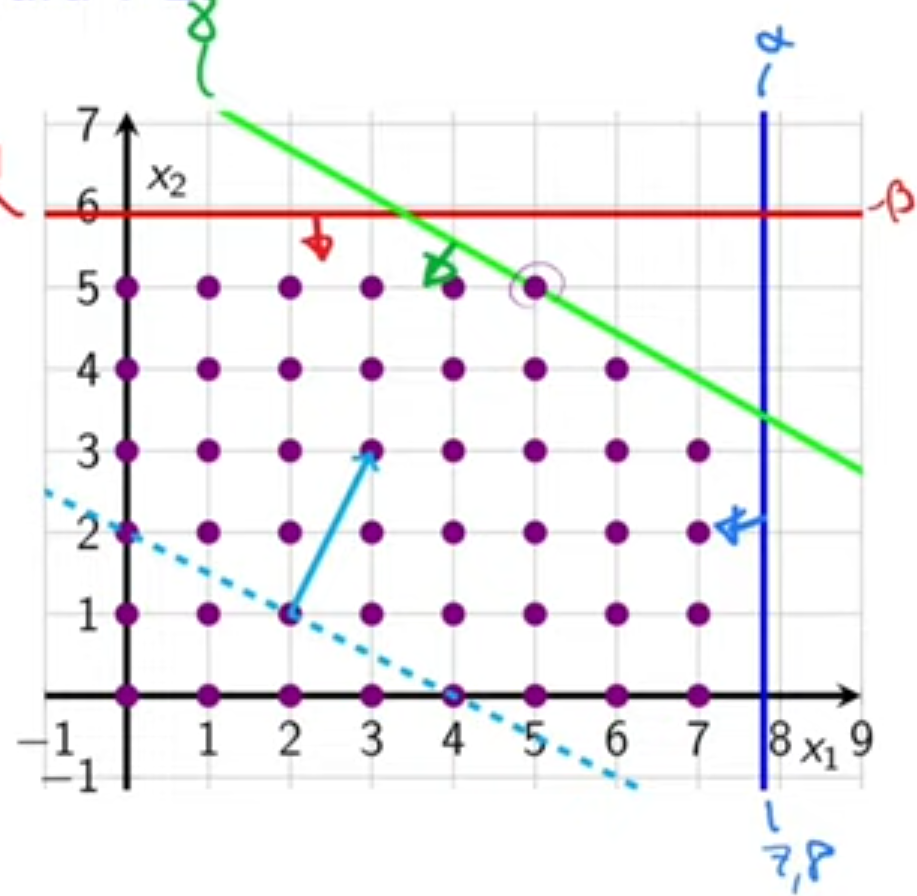
\includegraphics[width=.45\textwidth]{img/ex_branch_bound_1.png}
\end{multicols}

Para resolver o problema, primeiro relaxamos a integralidade do PLI ($x_1,x_2\in\mathbb{R}^+$) para encontrar o limitante dual das soluções através da solução de um problema de PL (através do Simplex, por exemplo).

Temos, por exemplo, como solução o ponto $(3,4; 5,9)$ com valor da função objetivo $15,2$. Com isso, a melhor solução (do PL) tem funçao objetivo $15,2$ como limitante dual (nenhuam solução do PLI vai ser melhor que isso).

Fazemos primeiro o \textit{branch} em torno da variáveis mais fracionária (em que o PL tem ``mais dúvida'').

\begin{center}
    \begin{tikzpicture}[every node/.style={fill=white}, n/.style={circle, draw}]
        \node[n] (1) at (0, 0) {15,2};
        \node[n] (2) [below left=of 1] {$x_1\leq3$};
        \node[n] (3) [below right=of 1] {$x_2\geq4$};

        \draw (1) edge (2);
        \draw (1) edge (3);
    \end{tikzpicture}
\end{center}

Agora temos dois subproblemas (dois novos polígonos) e repetimos o procedimento para cada novo subproblema (usamos o PL para calcular o limitante dual).

\begin{multicols}{2}

    \null \vfill
    \begin{center}
        \begin{tikzpicture}[every node/.style={fill=white}, n/.style={circle, draw}]
            \node[n] (1) at (0, 0) {15,2};
            \node[n, fill=violet!20] (2) [below left=of 1] {14,8};
            \node[n, fill=teal!20] (3) [below right=of 1] {15,125};
    
            \draw (1) edge node {$x_1\leq3$} (2);
            \draw (1) edge node {$x_1\geq4$} (3);
        \end{tikzpicture}
    \end{center}
    \vfill \null

    \columnbreak

    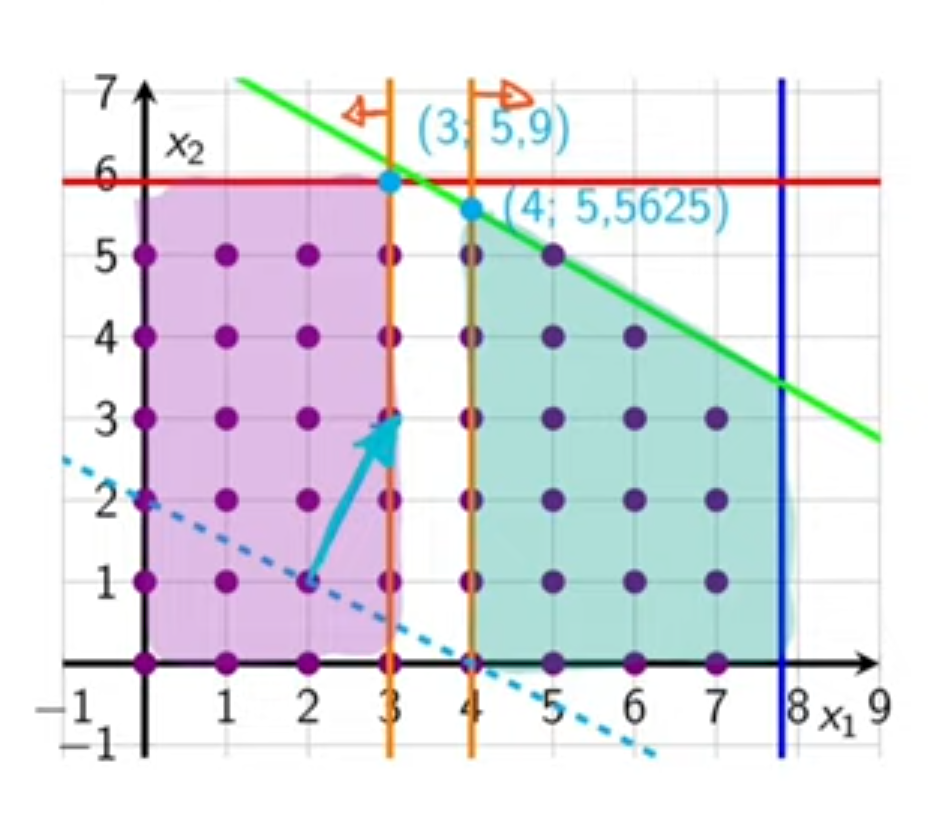
\includegraphics[width=.45\textwidth]{img/ex_branch_bound_2.png}
\end{multicols}

A partir daqui, podemos explorar seguindo aquele ramo que possui ``maior espaço para melhoria''. Ou seja, aquele cujo limitante dual esteja mais próximo do limitante dual original, nesse caso o ramo da direita. temos então como solução limitante $(4; 5,5625)$. $x_1$ não está fracionária, então fazemos a ramificação com a variável $x_2$.

\begin{center}
    \begin{tikzpicture}[every node/.style={fill=white}, n/.style={circle, draw}]
        \node[n] (1) at (0, 0) {15,2};
        \node[n] (2) [below left=of 1] {14,8};
        \node[n] (3) [below right=of 1] {15,125};
        \node[n] (4) [below left=of 3] {$x_2\leq5$};
        \node[n] (5) [below right=of 3] {$x_2\geq6$};

        \draw (1) edge node {$x_1\leq3$} (2);
        \draw (1) edge node {$x_1\geq4$} (3);
        \draw (3) edge (4);
        \draw (3) edge (5);
    \end{tikzpicture}
\end{center}

Com isso, temos:

\begin{multicols}{2}

    \null\vfill
    \begin{center}
        \begin{tikzpicture}[every node/.style={fill=white}, n/.style={circle, draw}]
            \node[n] (1) at (0, 0) {15,2};
            \node[forbidden sign, draw, fill=violet!20] (2) [below left=of 1] {14,8};
            \node[n] (3) [below right=of 1] {15,125};
            \node[n, fill=teal!20] (4) [below left=of 3] {15};
            \node[forbidden sign, draw] (5) [below right=of 3] {\phantom{X}};
    
            \draw (1) edge node {$x_1\leq3$} (2);
            \draw (1) edge node {$x_1\geq4$} (3);
            \draw (3) edge node {$x_2\leq5$} (4);
            \draw (3) edge node {$x_2\geq6$} (5);
        \end{tikzpicture}
    \end{center}
    \vfill\null

    \columnbreak

    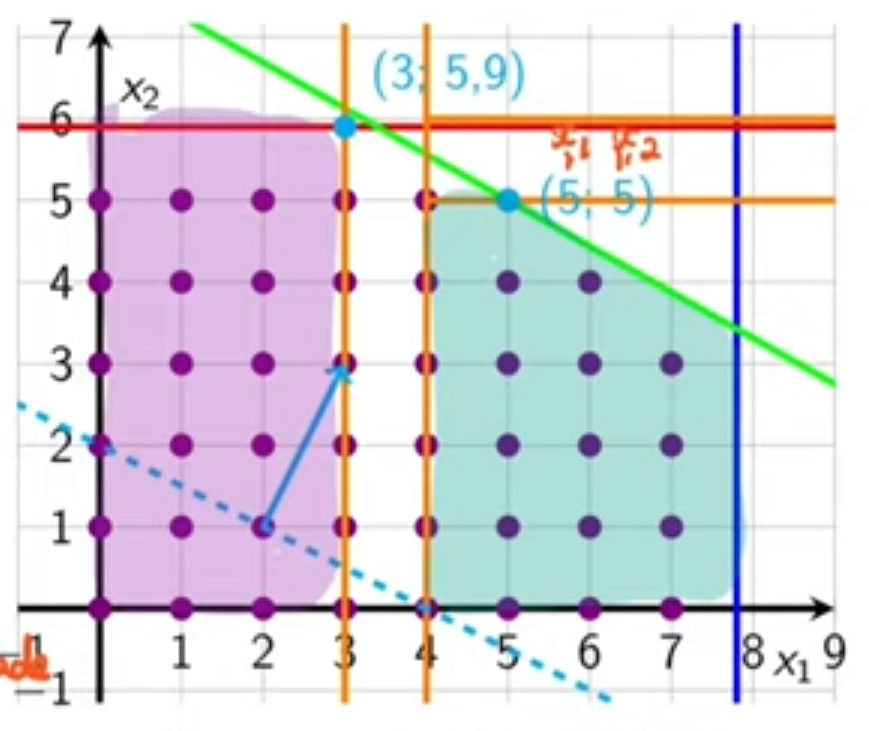
\includegraphics[width=.45\textwidth]{img/ex_branch_bound_3.png}
\end{multicols}

O ramo da direita não é mais explorado (é podado), pois temos uma inviabilidade, já que $x_2\geq6$ desrespeita a restrição $\beta$. Também não precisamos continuar explorando o ramo da esquerda, porque a solução do limitante dual já é inteira no ponto $(5; 5)$, então é a melhor solução inteira até o momento.

Deveríamos então continuar a explorar o subproblema em que $x_1\leq3$. Porém, sabemos que seu limitante dual é $14,8$, o que é menor que o valor da melhor solução inteira obtida (15), então não é necessário percorrer esse ramo, pois nunca terá uma solução melhor.

Como não temos mais nenhum nó ativo para ser percorrido, o algoritmo termina e temos como solução o ponto $(5; 5)$ com valor da função objetivo $15$.

\section{Pseudocódigo do Branch and Bound}

Enquanto houver \textbf{nós ativos}, escolher aquele com melhor (maximização/minimização) limitante dual.

\begin{itemize}
    \item Se o limitante dual for pior que a melhor solução já encontrada: eliminar o nó.
    \item Se a solução do PL desse nó for inteira, temos uma nova solução.
    \begin{itemize}
        \item Finalize o nó e atualize a melhor solução encontrada.
    \end{itemize}
    \item Caso contrário, ramifique o nó em torno da variável $x$ com valor $v$ mais fracionário (cuja parte decimal está mais perto de 0,5) na solução do PL.
    \begin{itemize}
        \item Crie dois subproblemas com $x\leq\lfloor v \rfloor$ e $x\geq\lceil v \rceil$
        \item Calcule o limitante dual do nó correspondente a cada subproblema
        \begin{itemize}
            \item Pode, por inviabilidade, podar aqueles que não tiverem solução
        \end{itemize}
    \end{itemize}
\end{itemize}

Antes de entrar no laço, calculamos o limitante dual do problema original e fazemos deste o primeiro nó.

\section{Problema da Mochila}

\begin{itemize}
    \item Variáveis: $x_i \in \{0,1\} \quad \forall i \in \{1,\dots,n\}$
    \item Função objetivo: $\max{\sum_{i=1}^nv_ix_i}$
    \item Restrição: $\sum_{i=1}^nw_ix_i\leq W$
\end{itemize}

Obtemos o PL, relaxando as restrições de integralidade $\to$ mochila fracionária.

O problema da mochila fracionária obtém a melhor solução através de um algoritmo guloso. Então podemos usar ele ao invés do Simplex.

\begin{example}
    \begin{itemize}
        \item $w_1=2\quad v_1=10\quad \frac{v_1}{w_1}=5$
        \item $w_2=3\quad v_2=21\quad \frac{v_2}{w_2}=7$
        \item $w_3=5\quad v_3=50\quad \frac{v_3}{w_2}=10$
        \item $w_4=7\quad v_4=51\quad \frac{v_4}{w_4}=8,5$
        \item $W = 7$
    \end{itemize}
\end{example}

Obtendo a melhor solução para o PL, usando o algoritmo guloso, temos que o limitante dual é: $v_3+\frac{2}{6}v_4=50+17=67$. A solução não é inteira, pois $x_4=\frac{1}{3}$. Ramificamos na variável mais fracionária ($x_4$).

\begin{example}
    \centering
    \begin{tikzpicture}[every node/.style={fill=white}, n/.style={ellipse, draw}]
        \node[n] (1) at (0, 0) {67};
        \node[n] (2) [below right=of 1] {$v_4+\frac{1}{5}v_3=61$};
        \node[n] (3) [below left=of 1] {$v_3+\frac{2}{3}v_2=64$};

        \draw (1) edge node {$x_4\geq1$} (2);
        \draw (1) edge node {$x_4\leq0$} (3);
    \end{tikzpicture}
\end{example}

Escolhemos o melhor limitante dual (como o problema é de maximização, pega-se o maior) e ramificamos de novo na variável mais fracionária ($x_2$). A restrição de que $x_4\leq 0$ continua valendo durante essa ramificação.

\begin{example}
    \centering
    \begin{tikzpicture}[every node/.style={fill=white}, n/.style={ellipse, draw}]
        \node[n] (1) at (0, 0) {67};
        \node[n] (2) [below right=of 1] {$61$};
        \node[n] (3) [below left=of 1] {$64$};
        \node[n] (4) [below right=of 3] {$v_2+\frac{4}{5}v_3=61$};
        \node[n] (5) [below left=of 3] {$v_3+v_1=60$};

        \draw (1) edge node {$x_4\geq1$} (2);
        \draw (1) edge node {$x_4\leq0$} (3);
        \draw (3) edge node {$x_2\geq1$} (4);
        \draw (3) edge node {$x_2\leq0$} (5);
    \end{tikzpicture}
\end{example}

Ramificamos novamente, o nó com limitante dual 61.

\begin{example}
    \centering
    \begin{tikzpicture}[every node/.style={fill=white}, n/.style={ellipse, draw}]
        \node[n] (1) at (0, 0) {67};
        \node[n] (2) [below right=of 1] {$61$};
        \node[n] (3) [below left=of 1] {$64$};
        \node[n] (4) [below right=of 3] {$61$};
        \node[n] (5) [below left=of 3] {$60$};
        \node[n] (6) [below right=of 4] {\sout{$w_2+w_3=8>7=W$}};
        \node[n] (7) [below left=of 4] {$v_2+v_1=31$};

        \draw (1) edge node {$x_4\geq1$} (2);
        \draw (1) edge node {$x_4\leq0$} (3);
        \draw (3) edge node {$x_2\geq1$} (4);
        \draw (3) edge node {$x_2\leq0$} (5);
        \draw (4) edge node {$x_3\geq1$} (6);
        \draw (4) edge node {$x_3\leq0$} (7);
    \end{tikzpicture}
\end{example}

Removemos o nó em que $x_3\geq1$ porque ao ter $x_2$ e $x_3$ inteiramente na mochila, o peso é excedido, então a solução não é viável. Seguimos ramificando no nó com o melhor limitante dual (61), em que $x_4\geq1$.

\begin{example}
    \centering
    \begin{tikzpicture}[every node/.style={fill=white}, n/.style={ellipse, draw}]
        \node[n] (1) at (0, 0) {67};
        \node[n] (2) [below right=of 1] {$61$};
        \node[n] (3) [below left=of 1] {$64$};
        \node[n] (4) [below right=of 3] {$61$};
        \node[n] (5) [below left=of 3] {$60$};
        \node[forbidden sign, draw, fill=red!20] (6) [below right=of 4] {\phantom{X}};
        \node[n] (7) [below left=of 4] {$31$};
        \node[n] (8) [right=2cm of 2] {\sout{$w_4 + w_3 = 11 > 7 = W$}};
        \node[n] (9) [below right=of 2] {$v_4+\frac{1}{3}v_2=51+7=58$};

        \draw (1) edge node {$x_4\geq1$} (2);
        \draw (1) edge node {$x_4\leq0$} (3);
        \draw (3) edge node {$x_2\geq1$} (4);
        \draw (3) edge node {$x_2\leq0$} (5);
        \draw (4) edge node {$x_3\geq1$} (6);
        \draw (4) edge node {$x_3\leq0$} (7);
        \draw (2) edge node {$x_3\geq1$} (8);
        \draw (2) edge node {$x_3\leq0$} (9);
    \end{tikzpicture}
\end{example}

Removemos mais um nó por inviabilidade. Continuamos explorando os nós ativos com maior limitante dual. Nesse caso, o de valor $60$, em que $x_4\leq0, x_2\leq0$. Nesse caso, a solução existente já é inteira. Com $x_3=1,x_1=1$ e limitante dual $60$. Portanto, essa é a melhor solução obtida até o momento, essa solução é chamada de \textbf{limitante primal}. Ele é desativado, por ser o melhor possível.

\begin{example}
    \centering
    \begin{tikzpicture}[every node/.style={fill=white}, n/.style={ellipse, draw}]
        \node[n] (1) at (0, 0) {67};
        \node[n] (2) [below right=of 1] {$61$};
        \node[n] (3) [below left=of 1] {$64$};
        \node[n] (4) [below right=of 3] {$61$};
        \node[n] (5) [below left=of 3, fill=green!20] {$60$};
        \node[forbidden sign, draw, fill=red!20] (6) [below right=of 4] {\phantom{X}};
        \node[n] (7) [below left=of 4] {$31$};
        \node[forbidden sign, draw, fill=red!20] (8) [right=2cm of 2] {\phantom{X}};
        \node[n] (9) [below right=of 2] {$58$};

        \draw (1) edge node {$x_4\geq1$} (2);
        \draw (1) edge node {$x_4\leq0$} (3);
        \draw (3) edge node {$x_2\geq1$} (4);
        \draw (3) edge node {$x_2\leq0$} (5);
        \draw (4) edge node {$x_3\geq1$} (6);
        \draw (4) edge node {$x_3\leq0$} (7);
        \draw (2) edge node {$x_3\geq1$} (8);
        \draw (2) edge node {$x_3\leq0$} (9);
    \end{tikzpicture}
\end{example}

Seguimos explorando os outros nós ativos em ordem. Seguindo o nó com limitante dual $58$. Como esse limitante é menor que o limitante primal encontrado anteriormente, o nó é apenas podado por limitante.

\begin{example}
    \centering
    \begin{tikzpicture}[every node/.style={fill=white}, n/.style={ellipse, draw}]
        \node[n] (1) at (0, 0) {67};
        \node[n] (2) [below right=of 1] {$61$};
        \node[n] (3) [below left=of 1] {$64$};
        \node[n] (4) [below right=of 3] {$61$};
        \node[n] (5) [below left=of 3, fill=green!20] {$60$};
        \node[forbidden sign, draw, fill=red!20] (6) [below right=of 4] {\phantom{X}};
        \node[n] (7) [below left=of 4] {$31$};
        \node[forbidden sign, draw, fill=red!20] (8) [right=2cm of 2] {\phantom{X}};
        \node[forbidden sign, draw, fill=red!20] (9) [below right=of 2] {$58$};

        \draw (1) edge node {$x_4\geq1$} (2);
        \draw (1) edge node {$x_4\leq0$} (3);
        \draw (3) edge node {$x_2\geq1$} (4);
        \draw (3) edge node {$x_2\leq0$} (5);
        \draw (4) edge node {$x_3\geq1$} (6);
        \draw (4) edge node {$x_3\leq0$} (7);
        \draw (2) edge node {$x_3\geq1$} (8);
        \draw (2) edge node {$x_3\leq0$} (9);
    \end{tikzpicture}
\end{example}

Em seguida, o nó com valor limitante 31 também é podado por limitante.

\begin{example}
    \centering
    \begin{tikzpicture}[every node/.style={fill=white}, n/.style={ellipse, draw}]
        \node[n] (1) at (0, 0) {67};
        \node[n] (2) [below right=of 1] {$61$};
        \node[n] (3) [below left=of 1] {$64$};
        \node[n] (4) [below right=of 3] {$61$};
        \node[n] (5) [below left=of 3, fill=green!20] {$60$};
        \node[forbidden sign, draw, fill=red!20] (6) [below right=of 4] {\phantom{X}};
        \node[forbidden sign, draw, fill=red!20] (7) [below left=of 4] {$31$};
        \node[forbidden sign, draw, fill=red!20] (8) [right=2cm of 2] {\phantom{X}};
        \node[forbidden sign, draw, fill=red!20] (9) [below right=of 2] {$58$};

        \draw (1) edge node {$x_4\geq1$} (2);
        \draw (1) edge node {$x_4\leq0$} (3);
        \draw (3) edge node {$x_2\geq1$} (4);
        \draw (3) edge node {$x_2\leq0$} (5);
        \draw (4) edge node {$x_3\geq1$} (6);
        \draw (4) edge node {$x_3\leq0$} (7);
        \draw (2) edge node {$x_3\geq1$} (8);
        \draw (2) edge node {$x_3\leq0$} (9);
    \end{tikzpicture}
\end{example}

\section{Eficiência do Branch and Bound}

A eficiência depende do número de podas, que depende de:

\begin{itemize}
    \item limitante primal (melhor solução encontrada até o momento)
    \item limitante dual (solução do PL relaxado para o nó sendo avaliado)
\end{itemize}

Então devemos encontrar \textbf{limitantes mais fortes}.

\textbf{Gap}: diferença entre o limitante primal e o limitante dual ``mais frouxo'' (melhor resultado) dos nós ativos. $\rightarrow$ \lstinline{RELATIVE_MIP_GAP}

\subsection{Fortalecendo limitantes primais}

Pode usar heurísticas e passar essa informação para o resolvedor de PLI. $\rightarrow$ \lstinline{SetHint}

Também é possível arrendondar a solução do PL para obter uma solução inteira. Tem que prestar atenção no sentido das desigualdades para saber se arredonda para cima ou para baixo. $\rightarrow$ Fazer isso abre mão de encontrar a solução ótima

É comum que resolvedores tenham como setar um \textit{callback} para chamar depois de encontrar a solução da relaxação. Pode usar isso para resolver o arredondamento. $\rightarrow$ Não tem no Or-tools, mas tem no Gurobi (pago)

Em geral, o valor de uma variável indica o quanto ela é ``interessante'' para a solução do problema.

\subsection{Fortalecendo limitantes duais}

O limitante dual é obtido da solução do PL vindo da relaxação. $\rightarrow$ Temos que melhorar a formulação do PL

Devemos encontrar \textbf{novas desigualdades} que \textbf{não} eliminam nenhuma solução \textbf{inteira} válida, mas que elimine soluções fracionárias da região viável. ``Diminui a área da região viável, aproximando as desigualdades do PL aos pontos inteiros''

Envoltória convexa, fecho convexo ou \textit{convex hull} $\rightarrow$ Menor conjunto convexo que possui todos os pontos de um conjunto. \textbf{Todo vértice é inteiro, desde que o conjunto só tenha pontos inteiros}.

Se encontrarmos a envoltória convexa do problema e executar a relaxação nesta área, vamos sempre obter a solução ótima. $\rightarrow$ Encontrar a envoltória convexa é NP-Difícil

\section{Problema do Conjunto Independente}

\begin{itemize}
    \item \textbf{Entrada:} grafo $G = (V, E)$
    \item \textbf{Soluções viáveis:} um conjunto $S \subseteq V$ tal que toda aresta $(u, v) \in E$ tem no máximo um extremo em $S$
    \item \textbf{Função objetivo:} tamanho de $S$
    \item \textbf{Objetivo:} encontrar solução de valor máximo
\end{itemize}

\subsection{Formulação em PLI para o Conjunto Independente}

\begin{itemize}
    \item Variáveis: $x_u \in \{0, 1\} \quad \forall u \in V$
    \item Função objetivo: $\max \sum_{u \in V}x_u$
    \item Restrição: $x_u + x_v \leq 1 \quad \forall (u, v) \in E$
\end{itemize}

Na relaxação: $0 \leq x_u \leq 1$.

\begin{example}
    \begin{center}
        \begin{tikzpicture}[every node/.style={fill=white}, n/.style={circle, draw}]
            \node[n] (a) at (0, 0) {a};
            \node[n] (b) [below right=of a] {b};
            \node[n] (c) [below left=of a] {c};

            \draw (a) edge (b);
            \draw (a) edge (c);
            \draw (c) edge (b);
        \end{tikzpicture}
    \end{center}
\end{example}

Se no exemplo $x_a = 0,5; x_b=0,5; x_c=0,5$. O limitante dual é $1,5$, enquanto o limitante primal é $1,0$.

Sabendo que o grafo é um triângulo (as arestas vão ter que ficar sozinhas em $S$), podemos criar uma outra restrição $x_a + x_b + x_c \leq 1$. Essa restrição não elimina nenhuma solução inteira, mas melhora as soluções do PL relaxado.

Isso pode servir a qualquer subgrafo completo (todos os nós conectados). $\rightarrow$ Clique


\end{document}